\begin{figure*}[!hbt]
  \centering
  \subfigure[Runtime on consecutive batch updates of size $10^{-5}|E_T|$]{
    \label{fig:temporal-sx-mathoverflow--runtime5}
    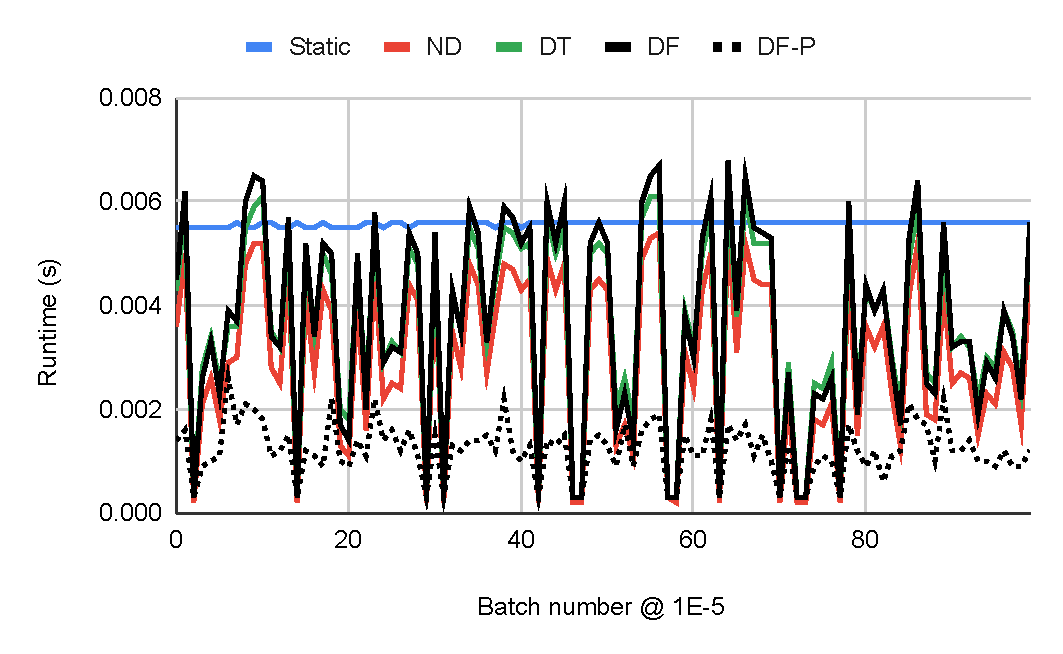
\includegraphics[width=0.48\linewidth]{out/temporal-sx-mathoverflow-runtime5.pdf}
  }
  \subfigure[Error in ranks obtained on consecutive batch updates of size $10^{-5}|E_T|$]{
    \label{fig:temporal-sx-mathoverflow--error5}
    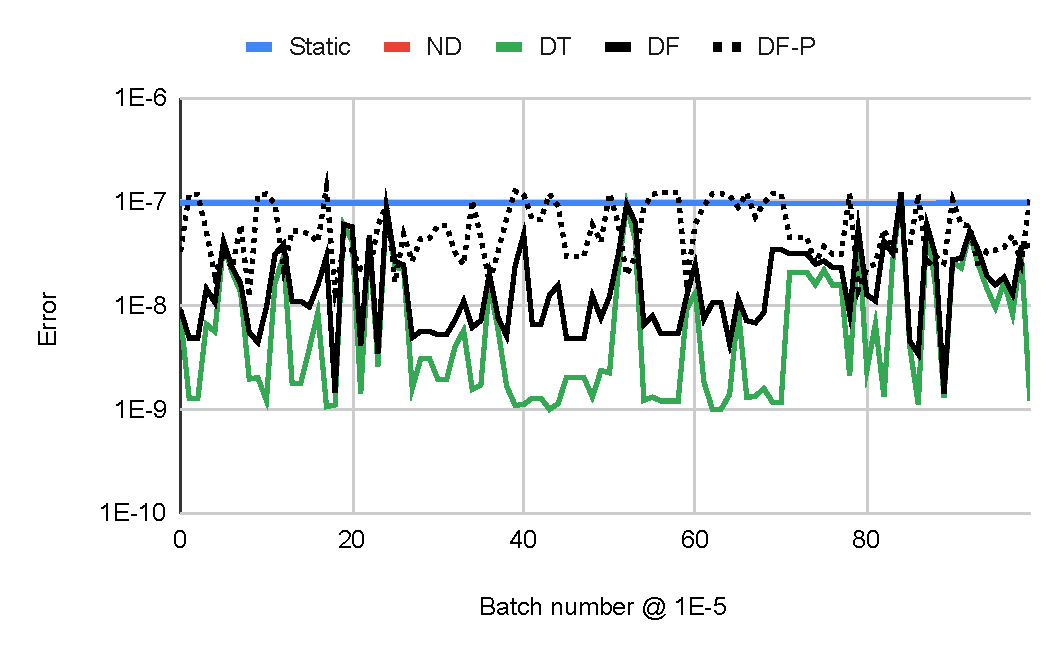
\includegraphics[width=0.48\linewidth]{out/temporal-sx-mathoverflow-error5.pdf}
  } \\[2ex]
  \subfigure[Runtime on consecutive batch updates of size $10^{-4}|E_T|$]{
    \label{fig:temporal-sx-mathoverflow--runtime4}
    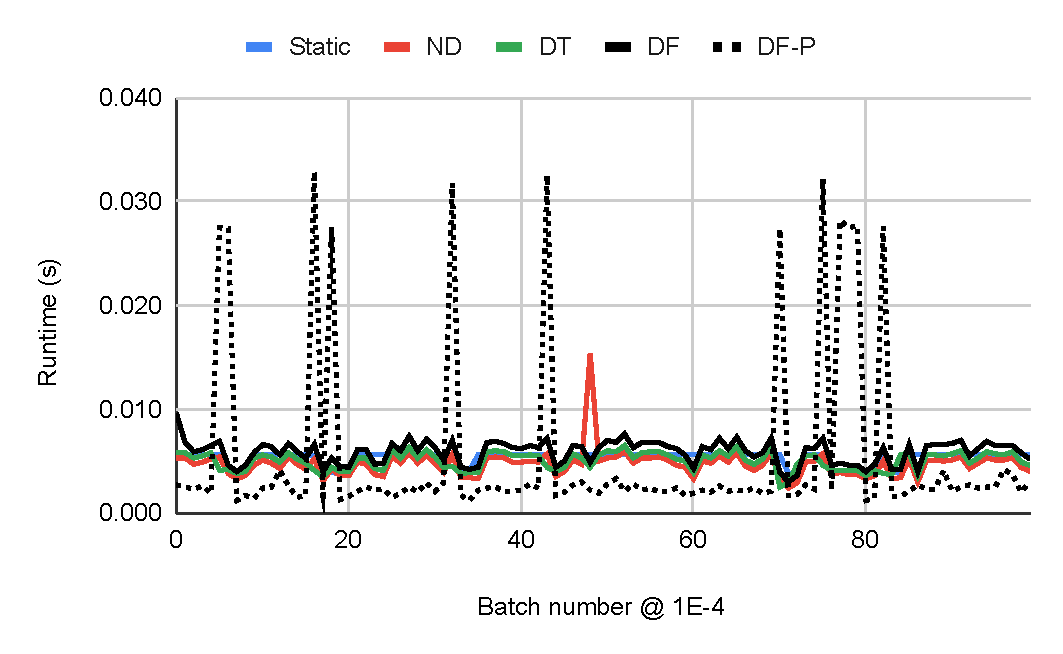
\includegraphics[width=0.48\linewidth]{out/temporal-sx-mathoverflow-runtime4.pdf}
  }
  \subfigure[Error in ranks obtained on consecutive batch updates of size $10^{-4}|E_T|$]{
    \label{fig:temporal-sx-mathoverflow--error4}
    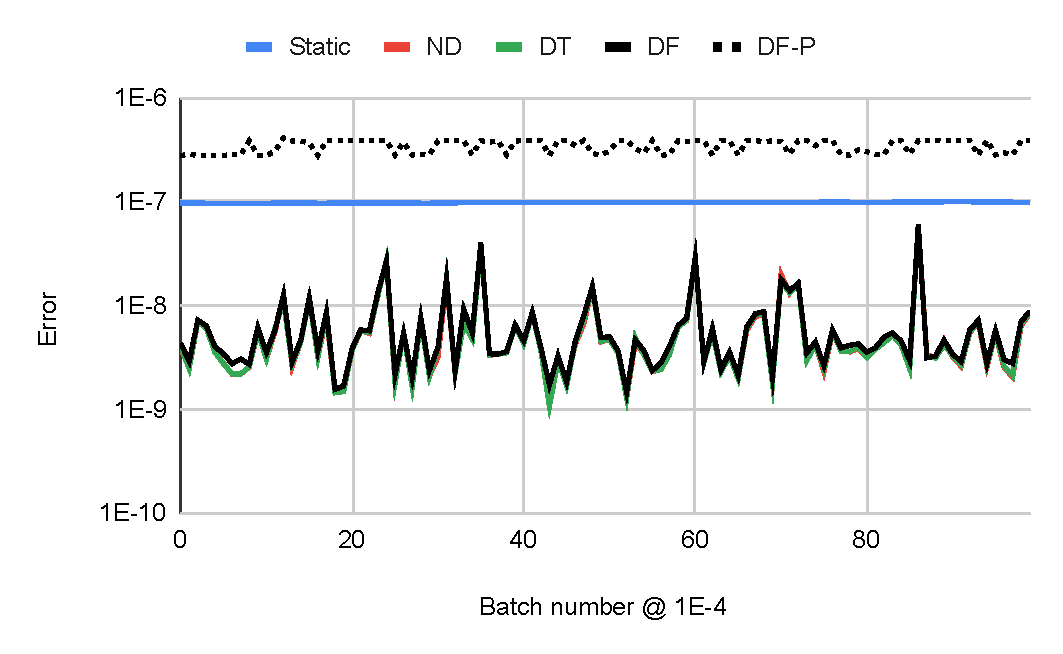
\includegraphics[width=0.48\linewidth]{out/temporal-sx-mathoverflow-error4.pdf}
  } \\[2ex]
  \subfigure[Runtime on consecutive batch updates of size $10^{-3}|E_T|$]{
    \label{fig:temporal-sx-mathoverflow--runtime3}
    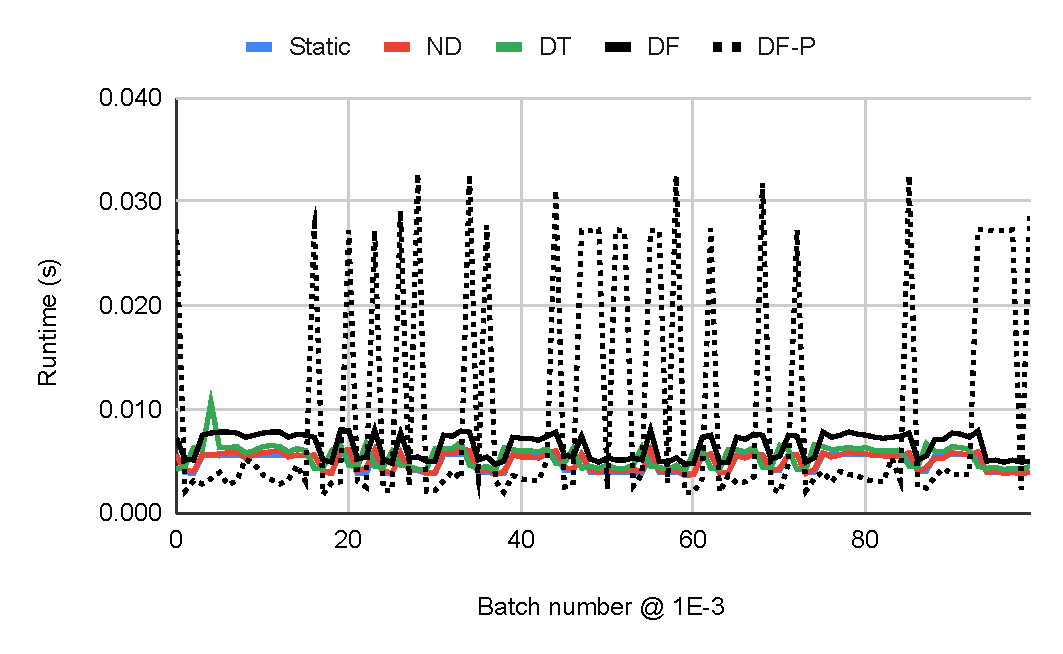
\includegraphics[width=0.48\linewidth]{out/temporal-sx-mathoverflow-runtime3.pdf}
  }
  \subfigure[Error in ranks obtained on consecutive batch updates of size $10^{-3}|E_T|$]{
    \label{fig:temporal-sx-mathoverflow--error3}
    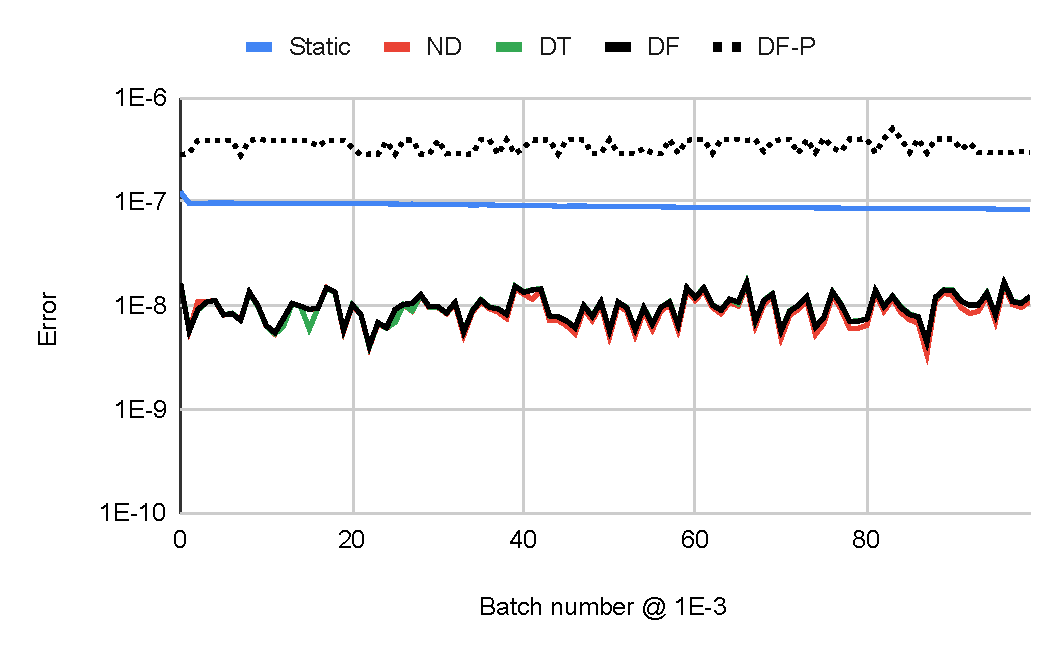
\includegraphics[width=0.48\linewidth]{out/temporal-sx-mathoverflow-error3.pdf}
  } \\[-2ex]
  \caption{Runtime and Error in ranks obtained with \textit{Static}, \textit{Naive-dynamic (ND)}, \textit{Dynamic Traversal (DT)}, our improved \textit{Dynamic Frontier (DF)}, and our improved \textit{Dynamic Frontier with Pruning (DF-P)} PageRank on the \textit{sx-mathoverflow} dynamic graph. The size of batch updates range from $10^{-5}|E_T|$ to $10^{-3}|E_T|$. The rank error with each approach is measured relative to ranks obtained with a reference Static PageRank run, as detailed in Section \ref{sec:measurement}. \su{TOWR}}
  \label{fig:temporal-sx-mathoverflow}
\end{figure*}

\begin{figure*}[!hbt]
  \centering
  \subfigure[Runtime on consecutive batch updates of size $10^{-5}|E_T|$]{
    \label{fig:temporal-sx-askubuntu--runtime5}
    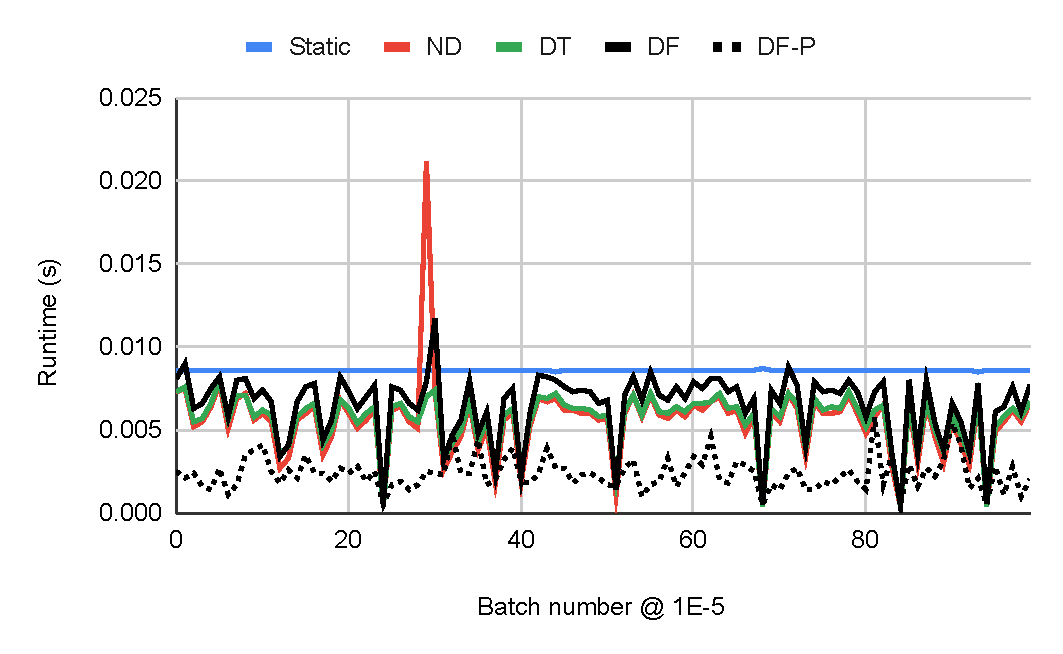
\includegraphics[width=0.48\linewidth]{out/temporal-sx-askubuntu-runtime5.pdf}
  }
  \subfigure[Error in ranks obtained on consecutive batch updates of size $10^{-5}|E_T|$]{
    \label{fig:temporal-sx-askubuntu--error5}
    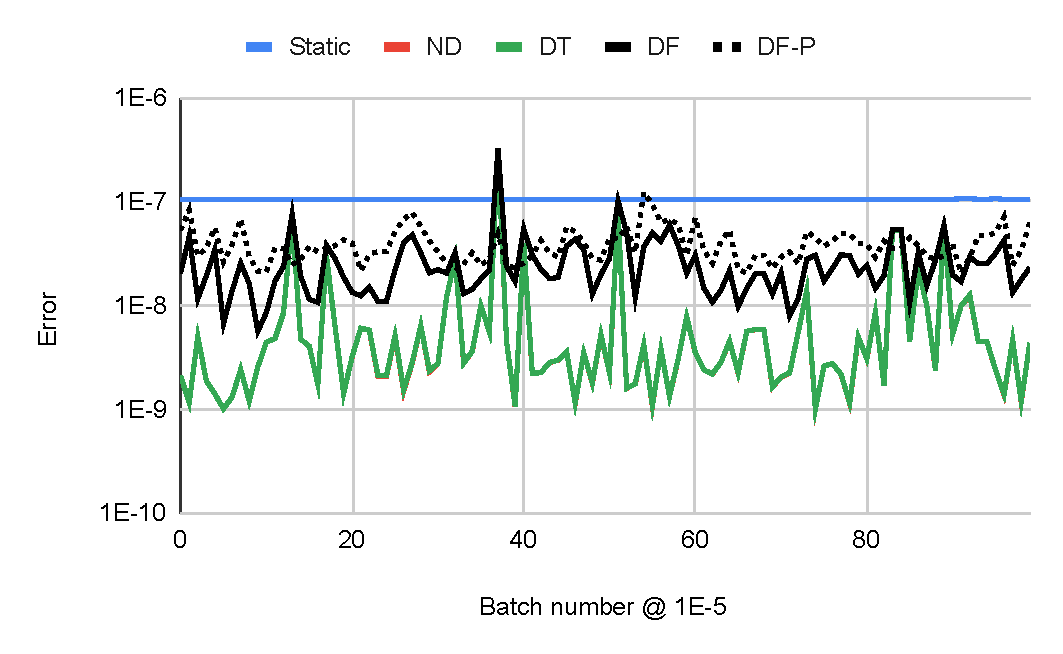
\includegraphics[width=0.48\linewidth]{out/temporal-sx-askubuntu-error5.pdf}
  } \\[2ex]
  \subfigure[Runtime on consecutive batch updates of size $10^{-4}|E_T|$]{
    \label{fig:temporal-sx-askubuntu--runtime4}
    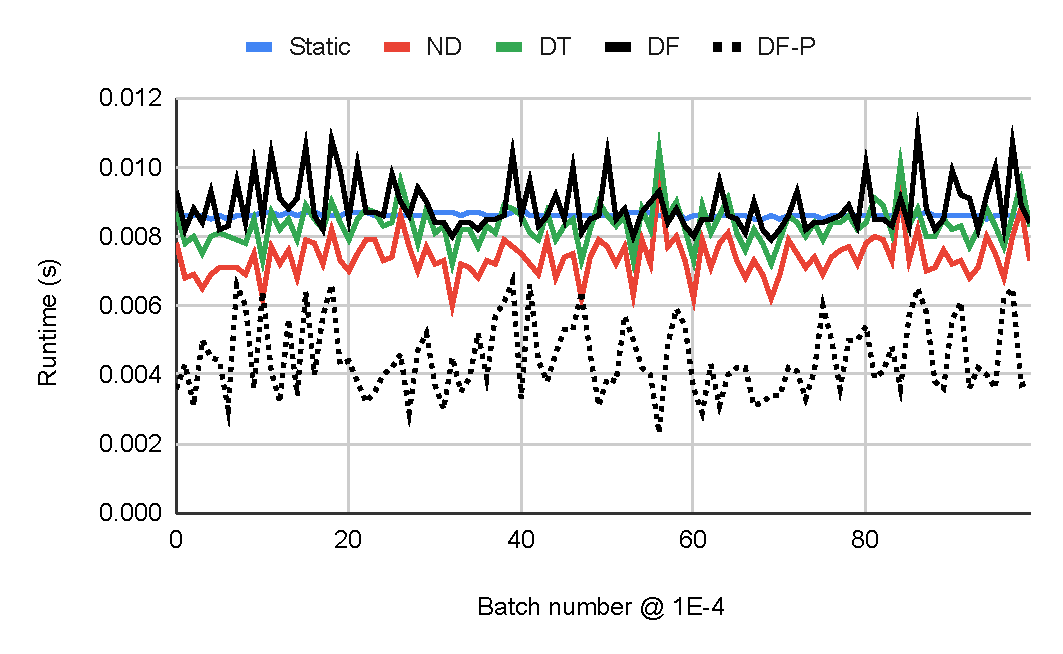
\includegraphics[width=0.48\linewidth]{out/temporal-sx-askubuntu-runtime4.pdf}
  }
  \subfigure[Error in ranks obtained on consecutive batch updates of size $10^{-4}|E_T|$]{
    \label{fig:temporal-sx-askubuntu--error4}
    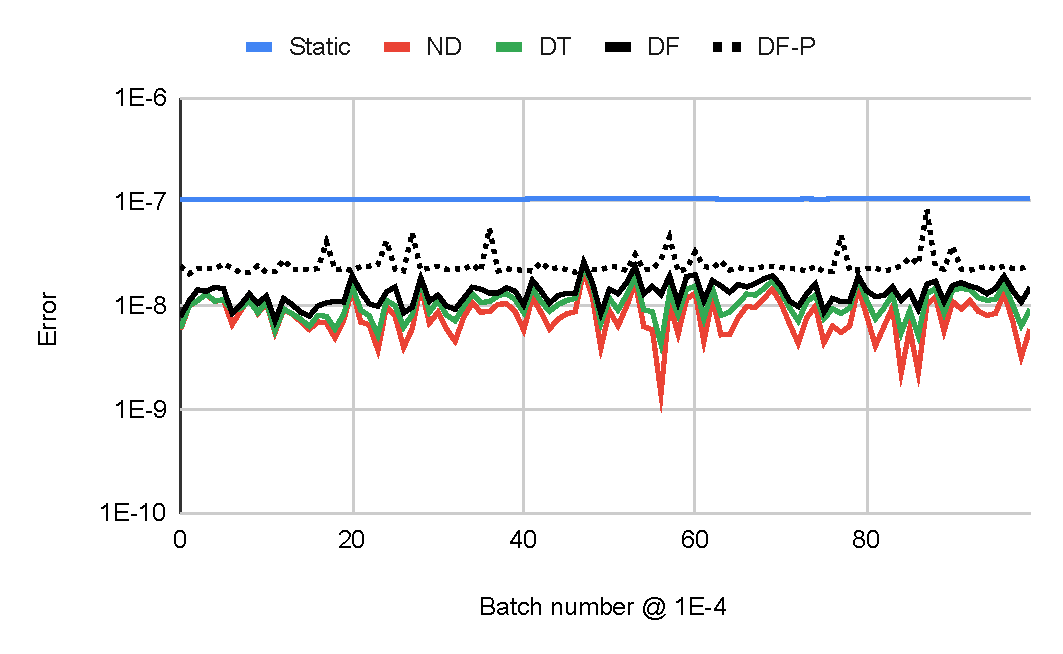
\includegraphics[width=0.48\linewidth]{out/temporal-sx-askubuntu-error4.pdf}
  } \\[2ex]
  \subfigure[Runtime on consecutive batch updates of size $10^{-3}|E_T|$]{
    \label{fig:temporal-sx-askubuntu--runtime3}
    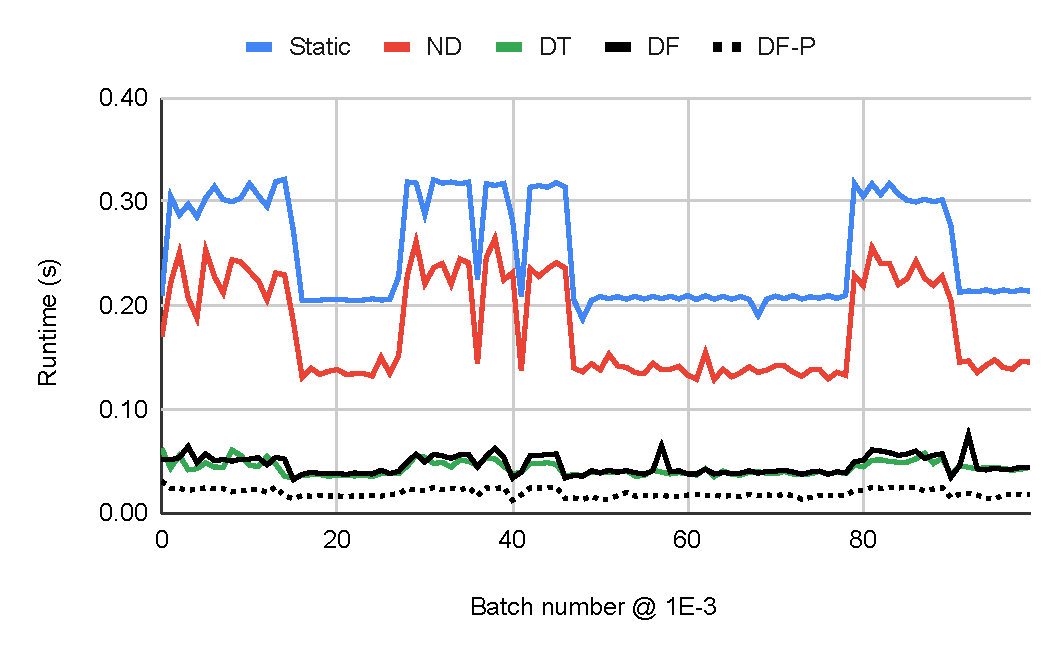
\includegraphics[width=0.48\linewidth]{out/temporal-sx-askubuntu-runtime3.pdf}
  }
  \subfigure[Error in ranks obtained on consecutive batch updates of size $10^{-3}|E_T|$]{
    \label{fig:temporal-sx-askubuntu--error3}
    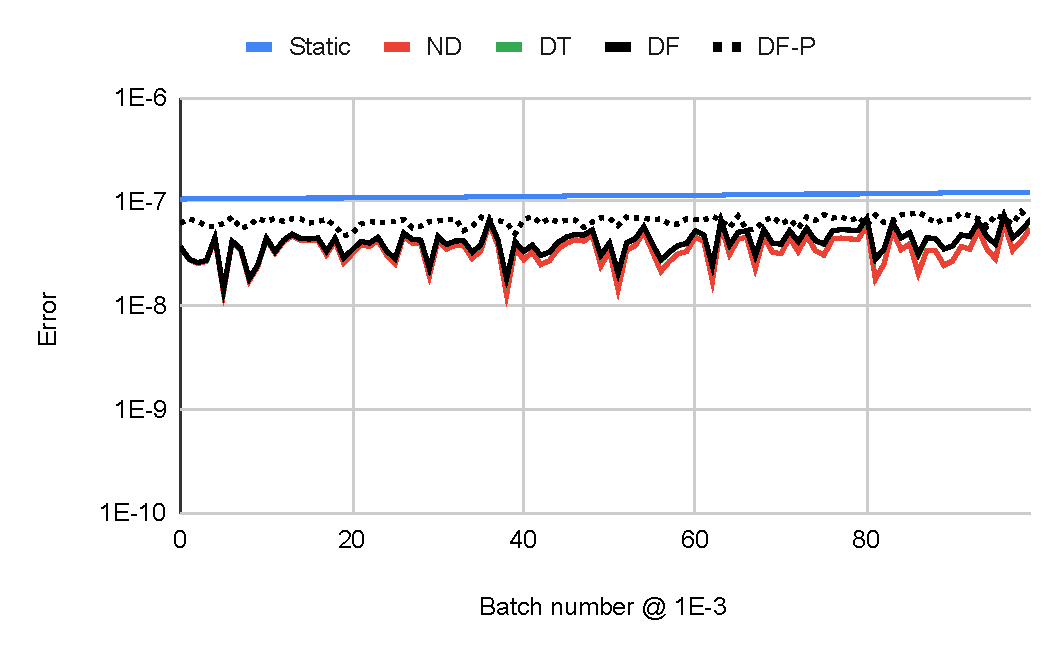
\includegraphics[width=0.48\linewidth]{out/temporal-sx-askubuntu-error3.pdf}
  } \\[-2ex]
  \caption{Runtime and Error in ranks obtained with our GPU implementation of \textit{Static}, \textit{Naive-dynamic (ND)}, \textit{Dynamic Traversal (DT)}, \textit{Dynamic Frontier (DF)}, and \textit{Dynamic Frontier with Pruning (DF-P)} PageRank on the \textit{sx-askubuntu} dynamic graph. The size of batch updates range from $10^{-5}|E_T|$ to $10^{-3}|E_T|$. The rank error with each approach is measured relative to ranks obtained with a reference Static PageRank run, as detailed in Section \ref{sec:measurement}.}
  \label{fig:temporal-sx-askubuntu}
\end{figure*}

\begin{figure*}[!hbt]
  \centering
  \subfigure[Runtime on consecutive batch updates of size $10^{-5}|E_T|$]{
    \label{fig:temporal-sx-superuser--runtime5}
    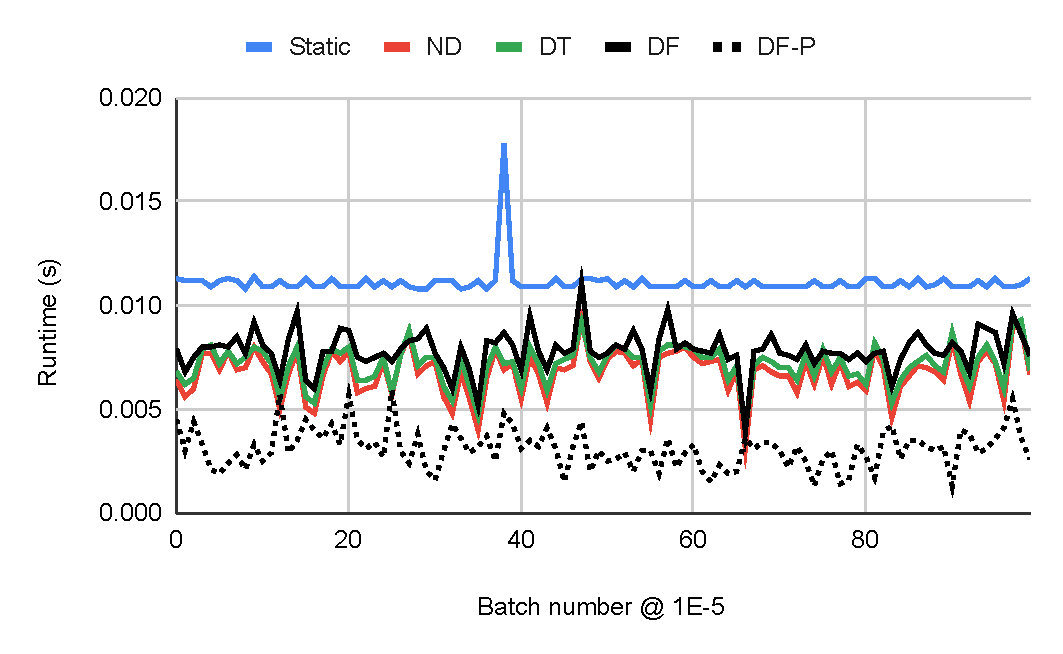
\includegraphics[width=0.48\linewidth]{out/temporal-sx-superuser-runtime5.pdf}
  }
  \subfigure[Error in ranks obtained on consecutive batch updates of size $10^{-5}|E_T|$]{
    \label{fig:temporal-sx-superuser--error5}
    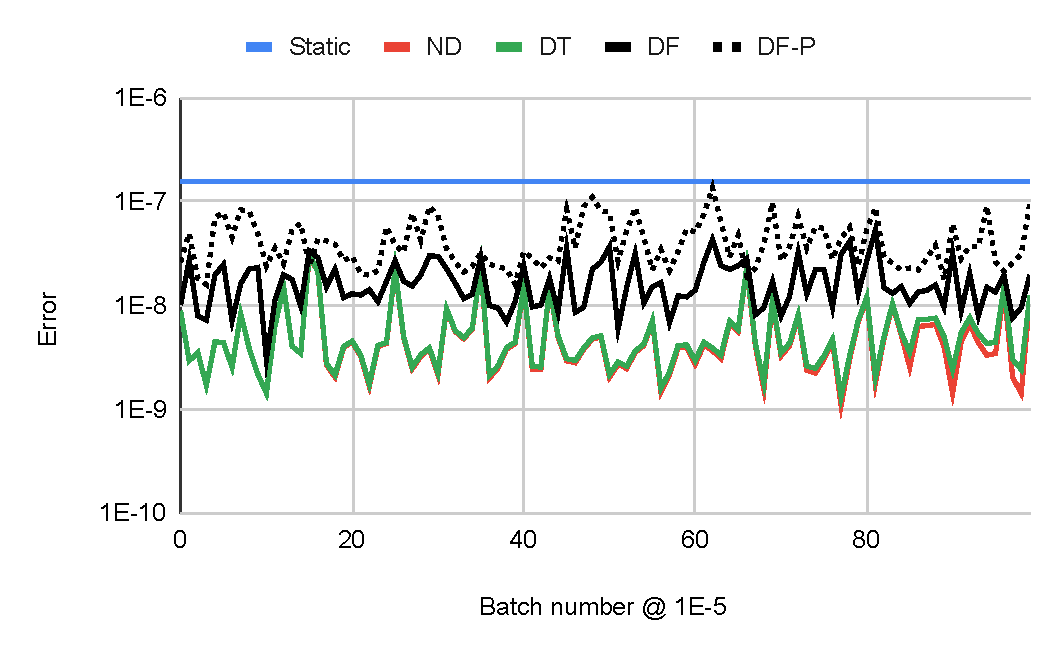
\includegraphics[width=0.48\linewidth]{out/temporal-sx-superuser-error5.pdf}
  } \\[2ex]
  \subfigure[Runtime on consecutive batch updates of size $10^{-4}|E_T|$]{
    \label{fig:temporal-sx-superuser--runtime4}
    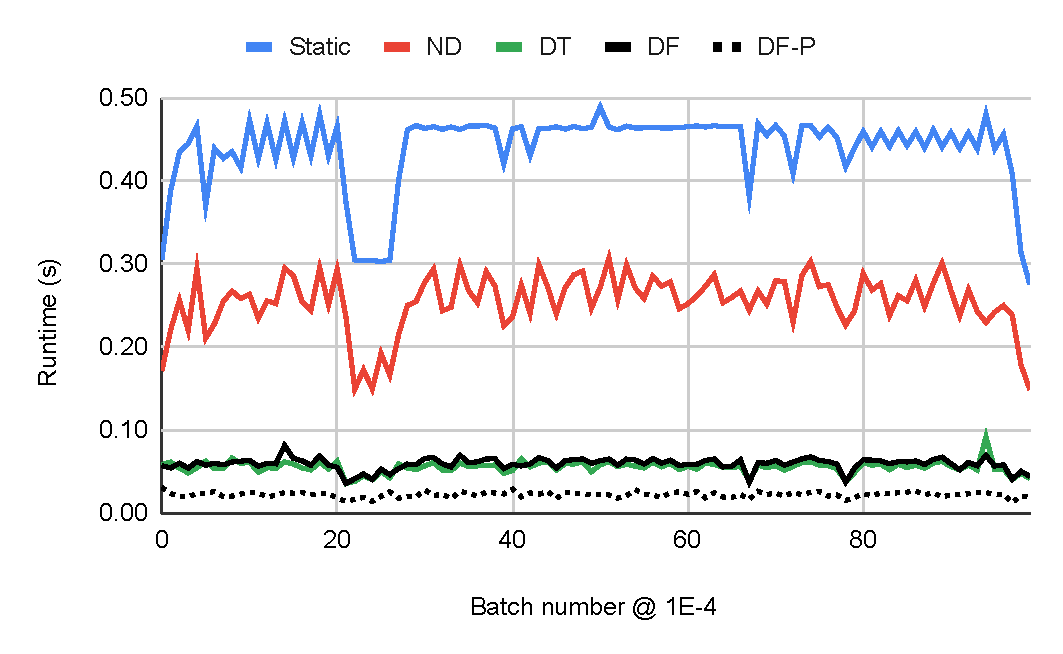
\includegraphics[width=0.48\linewidth]{out/temporal-sx-superuser-runtime4.pdf}
  }
  \subfigure[Error in ranks obtained on consecutive batch updates of size $10^{-4}|E_T|$]{
    \label{fig:temporal-sx-superuser--error4}
    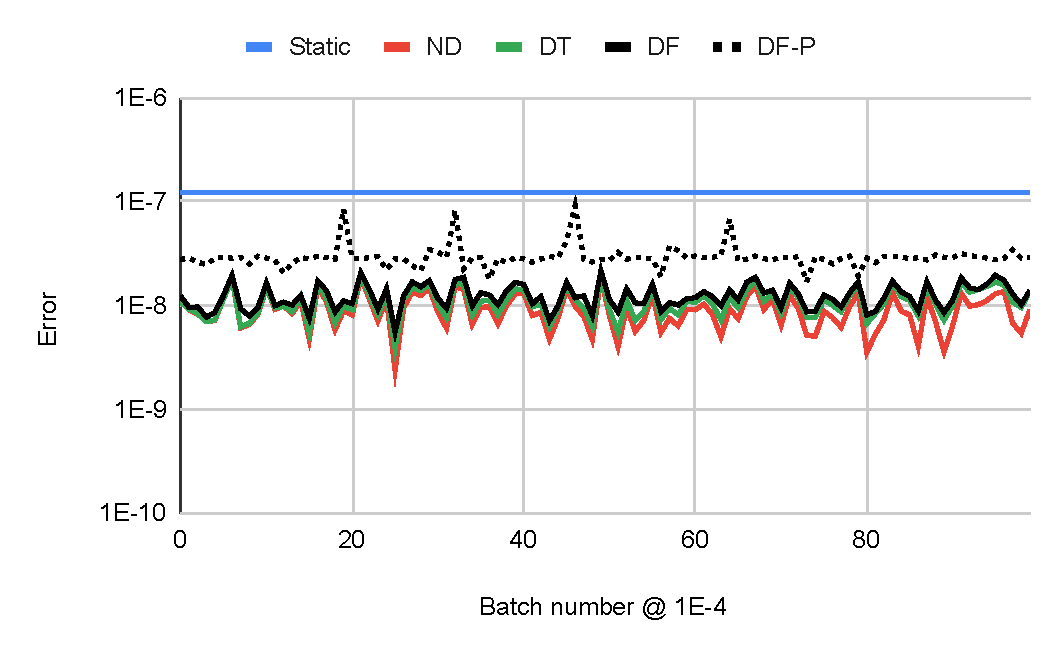
\includegraphics[width=0.48\linewidth]{out/temporal-sx-superuser-error4.pdf}
  } \\[2ex]
  \subfigure[Runtime on consecutive batch updates of size $10^{-3}|E_T|$]{
    \label{fig:temporal-sx-superuser--runtime3}
    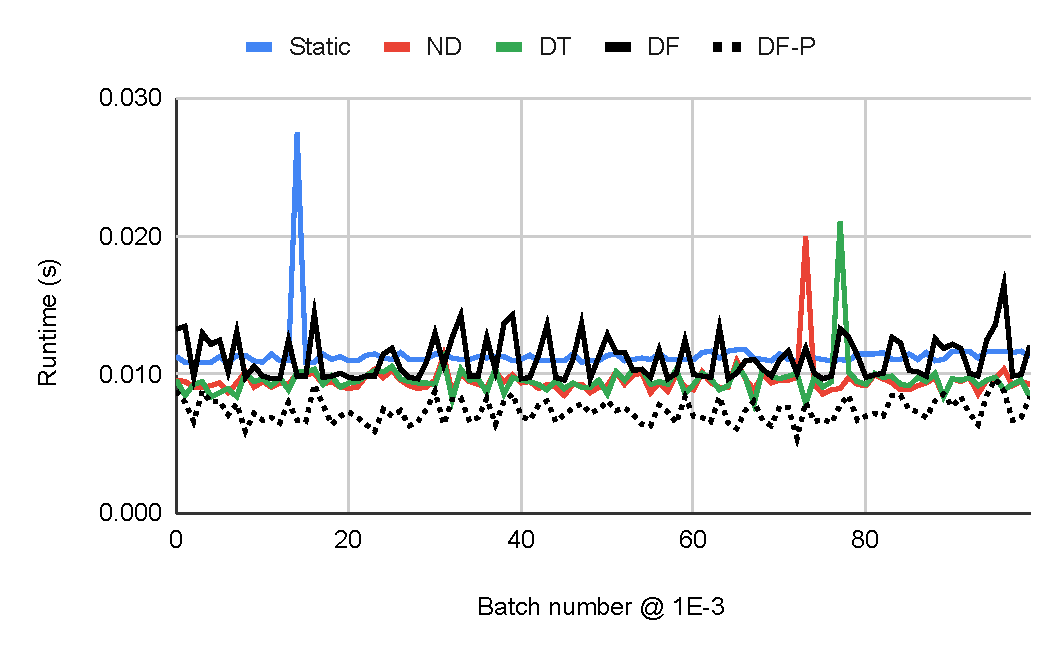
\includegraphics[width=0.48\linewidth]{out/temporal-sx-superuser-runtime3.pdf}
  }
  \subfigure[Error in ranks obtained on consecutive batch updates of size $10^{-3}|E_T|$]{
    \label{fig:temporal-sx-superuser--error3}
    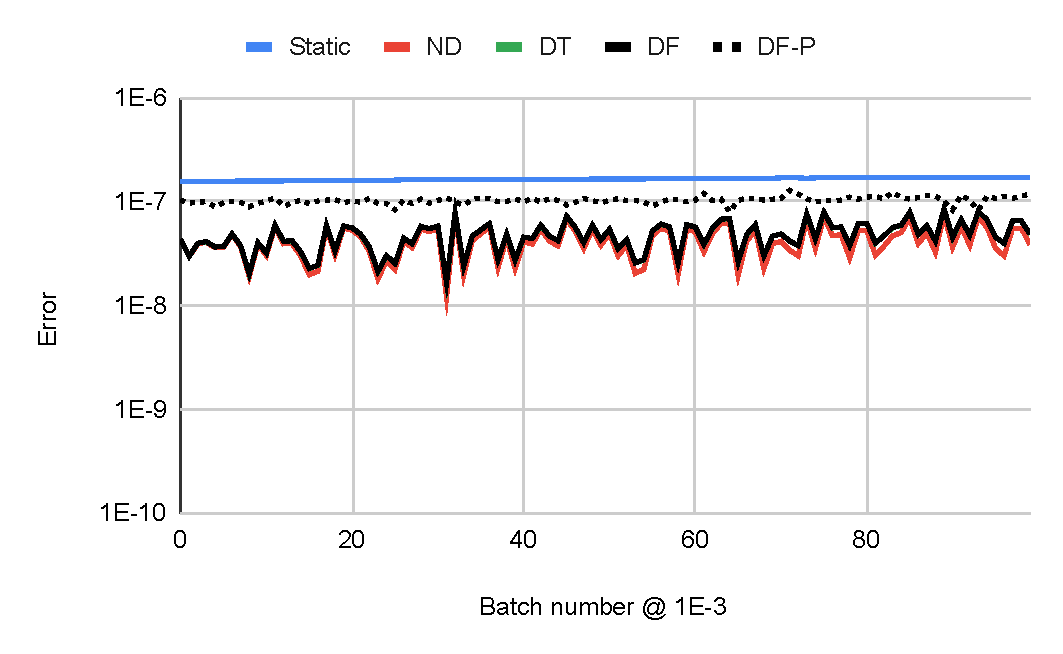
\includegraphics[width=0.48\linewidth]{out/temporal-sx-superuser-error3.pdf}
  } \\[-2ex]
  \caption{Runtime and Error in ranks obtained with \textit{Static}, \textit{Naive-dynamic (ND)}, \textit{Dynamic Traversal (DT)}, our improved \textit{Dynamic Frontier (DF)}, and our improved \textit{Dynamic Frontier with Pruning (DF-P)} PageRank on the \textit{sx-superuser} dynamic graph. The size of batch updates range from $10^{-5}|E_T|$ to $10^{-3}|E_T|$. The rank error with each approach is measured relative to ranks obtained with a reference Static PageRank run, as detailed in Section \ref{sec:measurement}.}
  \label{fig:temporal-sx-superuser}
\end{figure*}

\begin{figure*}[!hbt]
  \centering
  \subfigure[Runtime on consecutive batch updates of size $10^{-5}|E_T|$]{
    \label{fig:temporal-wiki-talk-temporal--runtime5}
    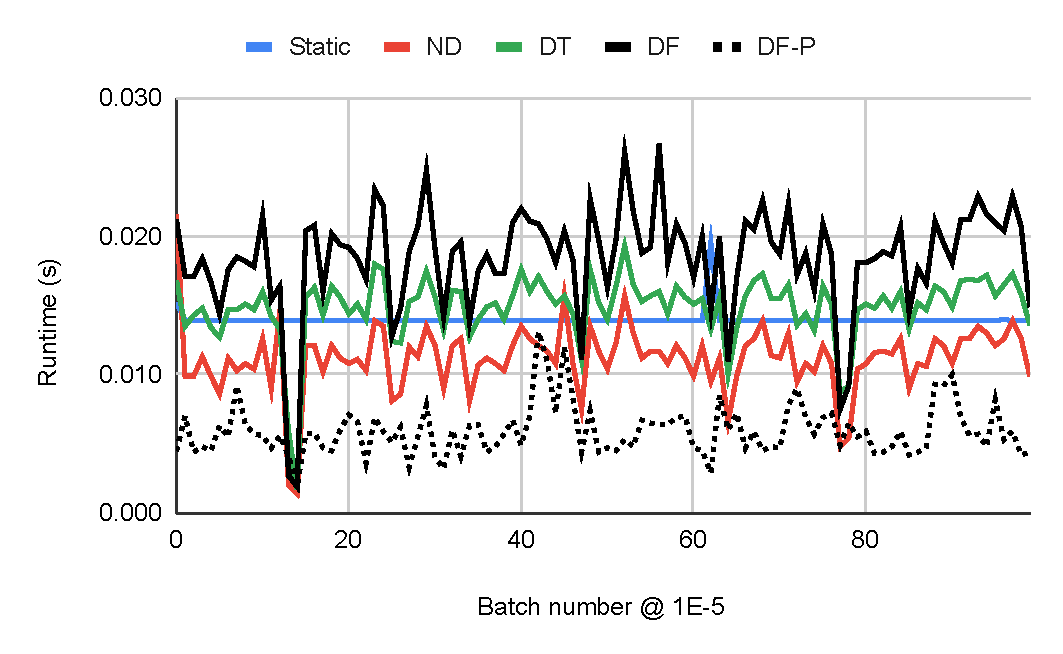
\includegraphics[width=0.48\linewidth]{out/temporal-wiki-talk-temporal-runtime5.pdf}
  }
  \subfigure[Error in ranks obtained on consecutive batch updates of size $10^{-5}|E_T|$]{
    \label{fig:temporal-wiki-talk-temporal--error5}
    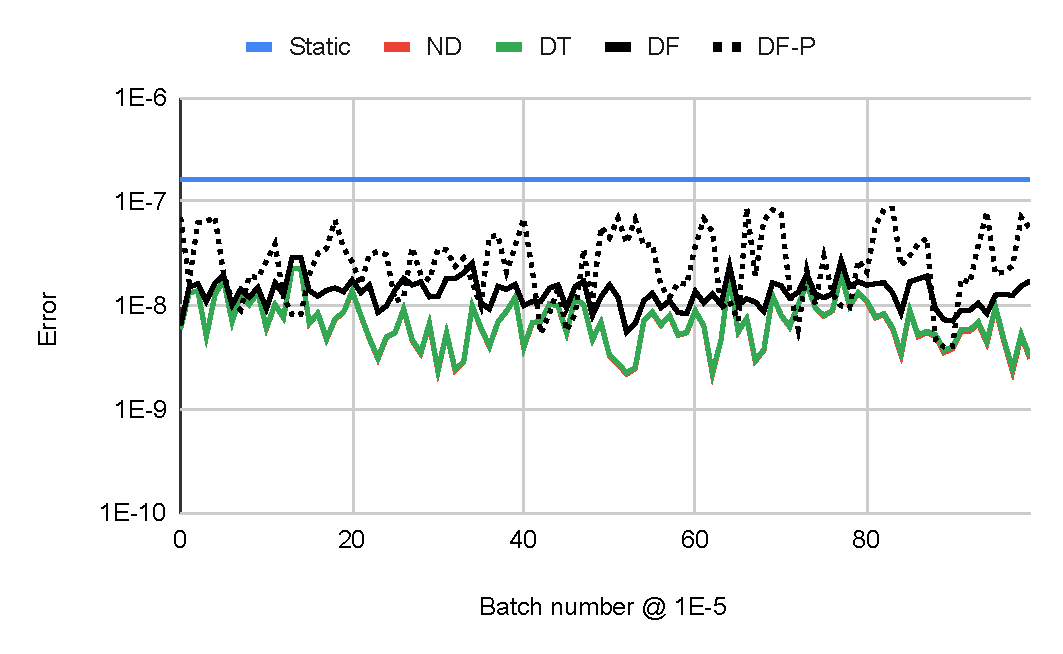
\includegraphics[width=0.48\linewidth]{out/temporal-wiki-talk-temporal-error5.pdf}
  } \\[2ex]
  \subfigure[Runtime on consecutive batch updates of size $10^{-4}|E_T|$]{
    \label{fig:temporal-wiki-talk-temporal--runtime4}
    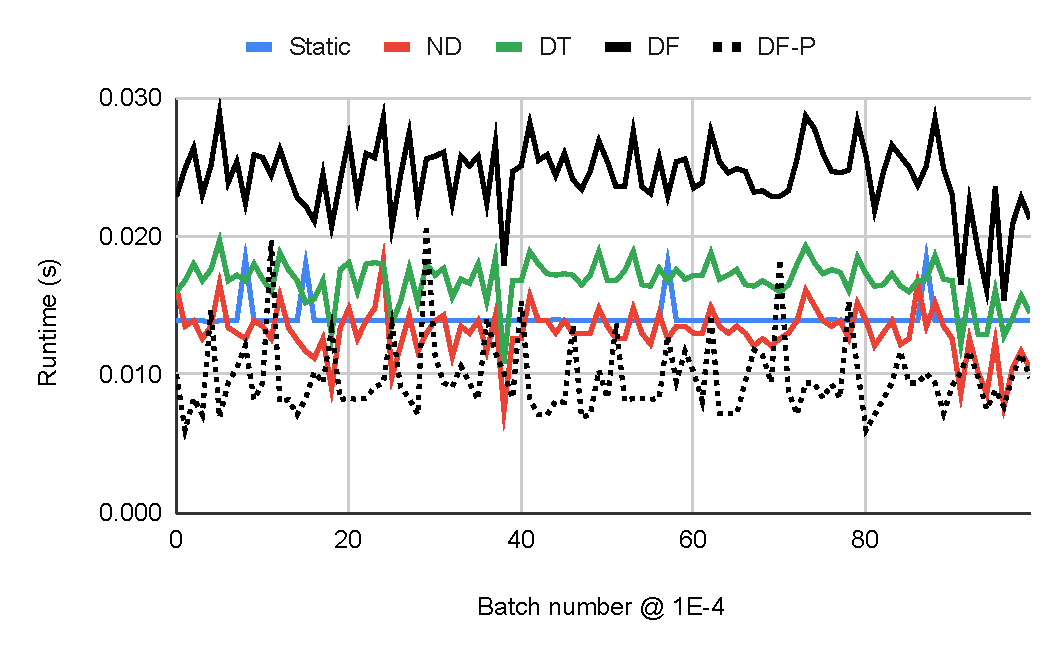
\includegraphics[width=0.48\linewidth]{out/temporal-wiki-talk-temporal-runtime4.pdf}
  }
  \subfigure[Error in ranks obtained on consecutive batch updates of size $10^{-4}|E_T|$]{
    \label{fig:temporal-wiki-talk-temporal--error4}
    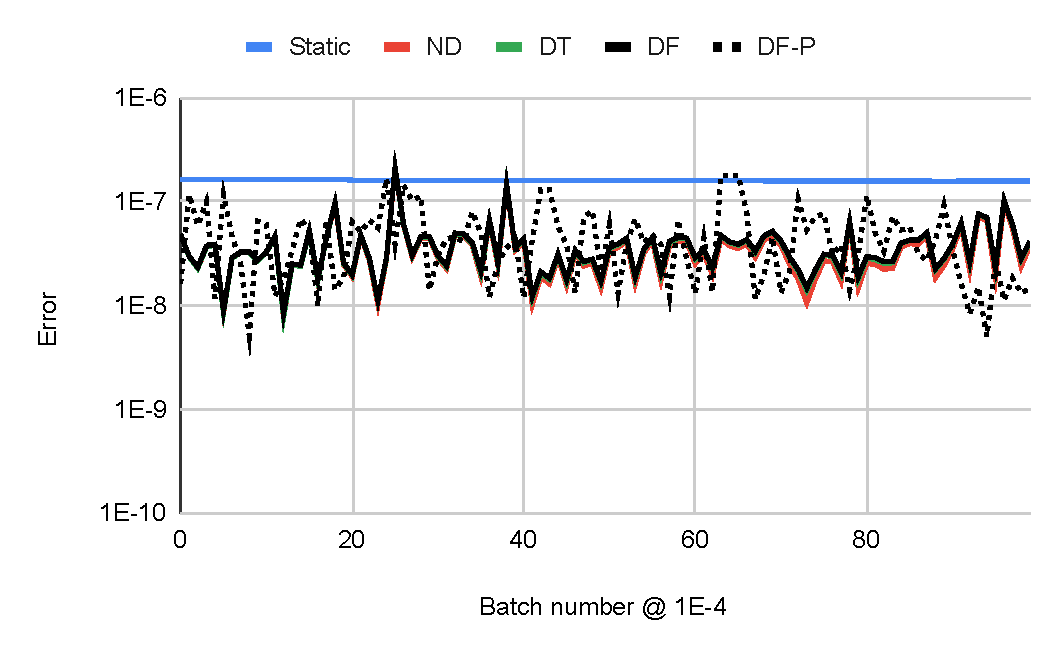
\includegraphics[width=0.48\linewidth]{out/temporal-wiki-talk-temporal-error4.pdf}
  } \\[2ex]
  \subfigure[Runtime on consecutive batch updates of size $10^{-3}|E_T|$]{
    \label{fig:temporal-wiki-talk-temporal--runtime3}
    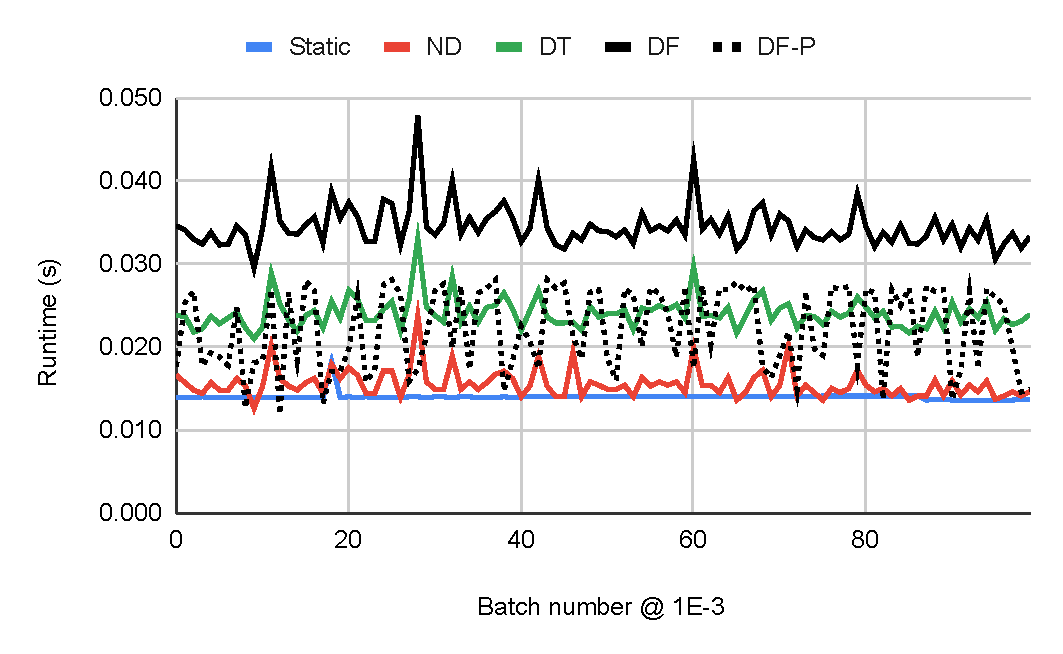
\includegraphics[width=0.48\linewidth]{out/temporal-wiki-talk-temporal-runtime3.pdf}
  }
  \subfigure[Error in ranks obtained on consecutive batch updates of size $10^{-3}|E_T|$]{
    \label{fig:temporal-wiki-talk-temporal--error3}
    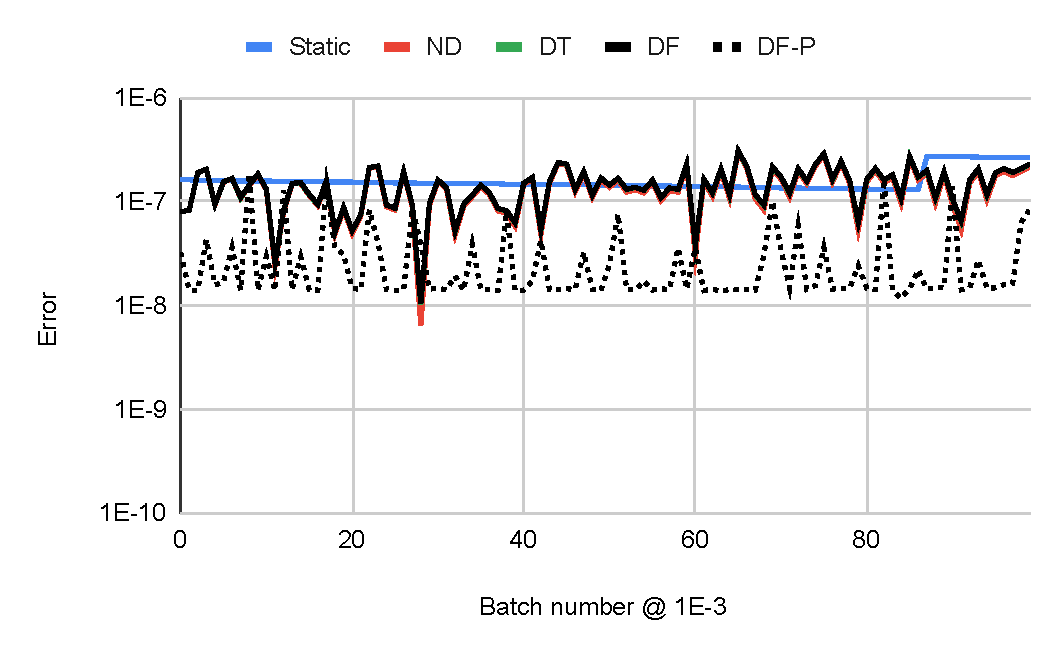
\includegraphics[width=0.48\linewidth]{out/temporal-wiki-talk-temporal-error3.pdf}
  } \\[-2ex]
  \caption{Runtime and Error in ranks obtained with our GPU implementation of \textit{Static}, \textit{Naive-dynamic (ND)}, \textit{Dynamic Traversal (DT)}, \textit{Dynamic Frontier (DF)}, and \textit{Dynamic Frontier with Pruning (DF-P)} PageRank on the \textit{wiki-talk-temporal} dynamic graph. The size of batch updates range from $10^{-5}|E_T|$ to $10^{-3}|E_T|$. The rank error with each approach is measured relative to ranks obtained with a reference Static PageRank run, as detailed in Section \ref{sec:measurement}.}
  \label{fig:temporal-wiki-talk-temporal}
\end{figure*}

\begin{figure*}[!hbt]
  \centering
  \subfigure[Runtime on consecutive batch updates of size $10^{-5}|E_T|$]{
    \label{fig:temporal-sx-stackoverflow--runtime5}
    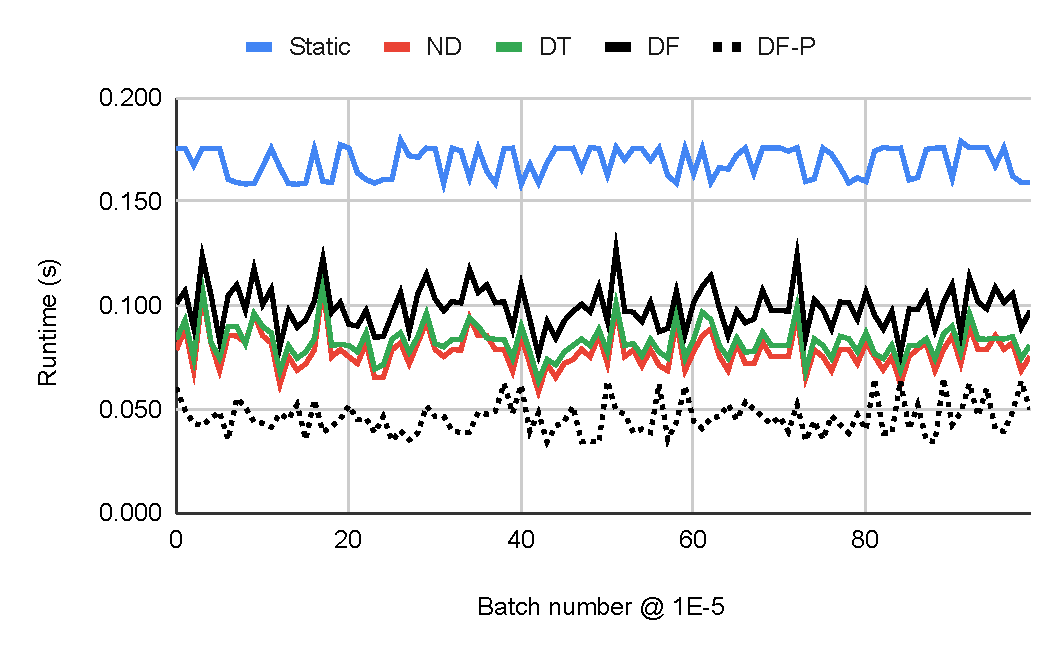
\includegraphics[width=0.48\linewidth]{out/temporal-sx-stackoverflow-runtime5.pdf}
  }
  \subfigure[Error in ranks obtained on consecutive batch updates of size $10^{-5}|E_T|$]{
    \label{fig:temporal-sx-stackoverflow--error5}
    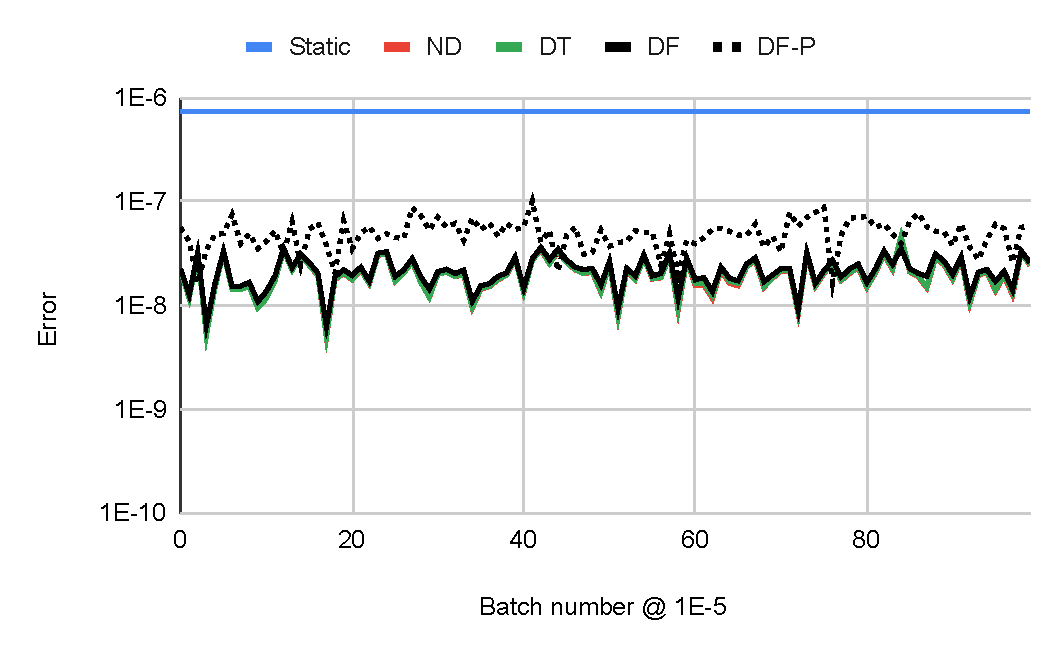
\includegraphics[width=0.48\linewidth]{out/temporal-sx-stackoverflow-error5.pdf}
  } \\[2ex]
  \subfigure[Runtime on consecutive batch updates of size $10^{-4}|E_T|$]{
    \label{fig:temporal-sx-stackoverflow--runtime4}
    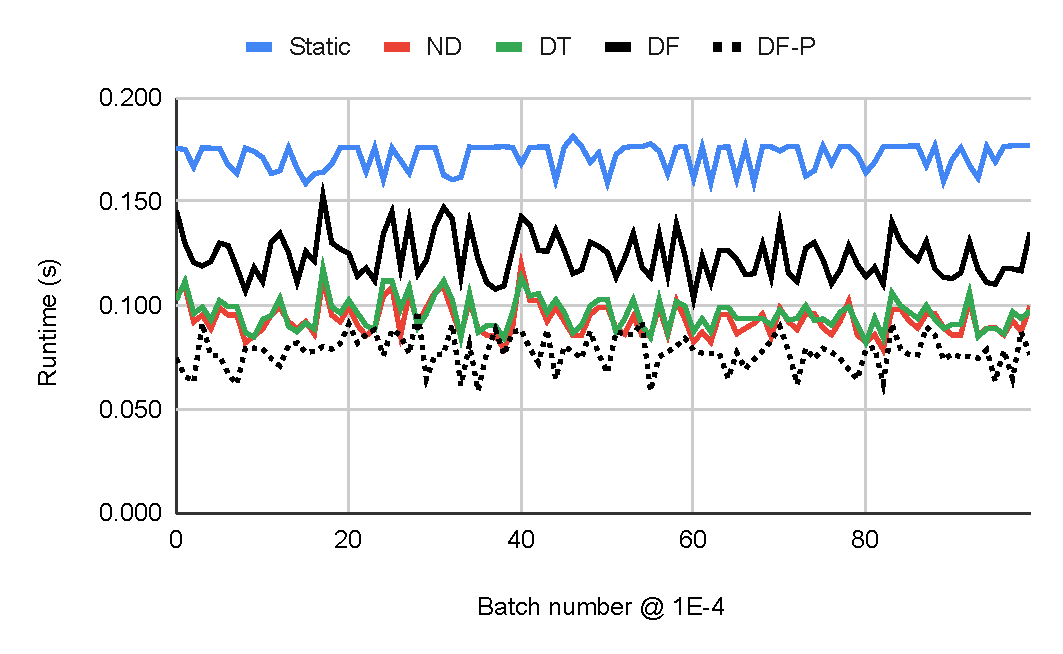
\includegraphics[width=0.48\linewidth]{out/temporal-sx-stackoverflow-runtime4.pdf}
  }
  \subfigure[Error in ranks obtained on consecutive batch updates of size $10^{-4}|E_T|$]{
    \label{fig:temporal-sx-stackoverflow--error4}
    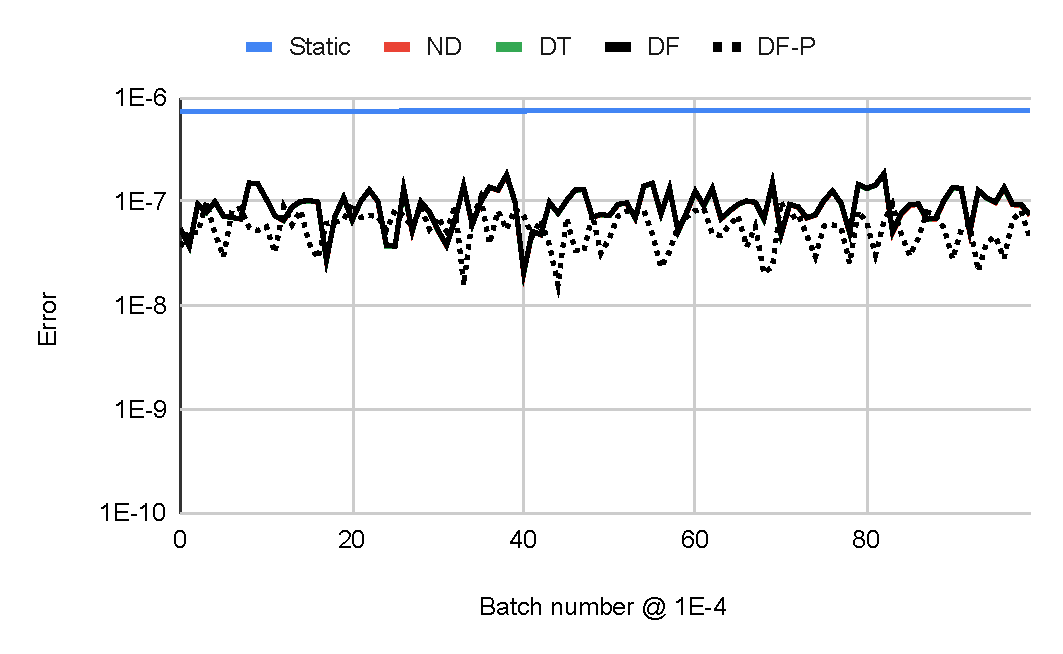
\includegraphics[width=0.48\linewidth]{out/temporal-sx-stackoverflow-error4.pdf}
  } \\[2ex]
  \subfigure[Runtime on consecutive batch updates of size $10^{-3}|E_T|$]{
    \label{fig:temporal-sx-stackoverflow--runtime3}
    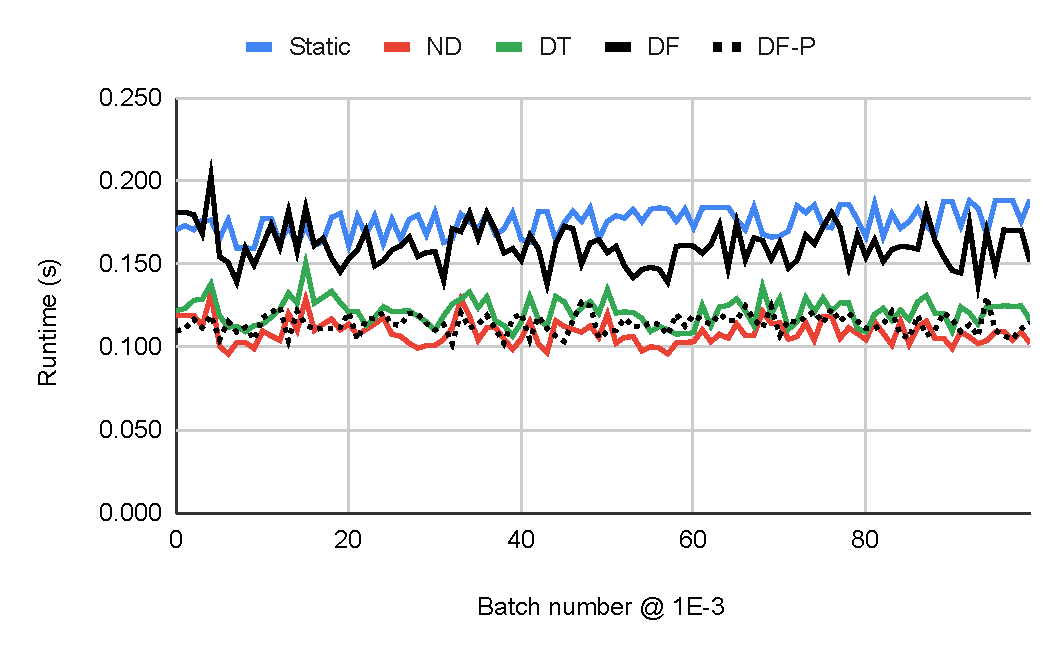
\includegraphics[width=0.48\linewidth]{out/temporal-sx-stackoverflow-runtime3.pdf}
  }
  \subfigure[Error in ranks obtained on consecutive batch updates of size $10^{-3}|E_T|$]{
    \label{fig:temporal-sx-stackoverflow--error3}
    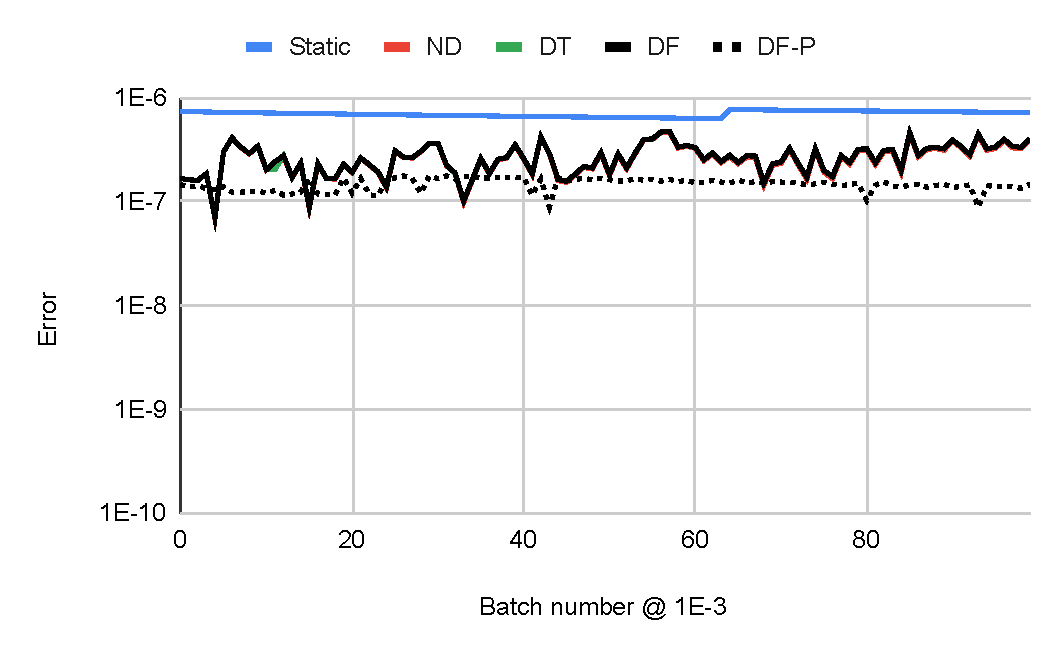
\includegraphics[width=0.48\linewidth]{out/temporal-sx-stackoverflow-error3.pdf}
  } \\[-2ex]
  \caption{Runtime and Error in ranks obtained with \textit{Static}, \textit{Naive-dynamic (ND)}, \textit{Dynamic Traversal (DT)}, our improved \textit{Dynamic Frontier (DF)}, and our improved \textit{Dynamic Frontier with Pruning (DF-P)} PageRank on the \textit{sx-stackoverflow} dynamic graph. The size of batch updates range from $10^{-5}|E_T|$ to $10^{-3}|E_T|$. The rank error with each approach is measured relative to ranks obtained with a reference Static PageRank run, as detailed in Section \ref{sec:measurement}. \su{TOWR}}
  \label{fig:temporal-sx-stackoverflow}
\end{figure*}


\clearpage

\section{Appendix}

\subsection{Derivation of Closed loop formula for Rank calculation towards Dynamic Frontier with Pruning (DF-P) PageRank}
\label{sec:pr-prune-derivation}

We proceed to derive the closed-loop formula for rank calculation with DF-P PageRank. As outlined in Sections \ref{sec:dataset} and \ref{sec:batch-generation}, self-loops are added to each vertex to circumvent the need for a global teleport rank computation in every iteration, thus reducing overhead. In DF-P PageRank, our aim is to skip the computation of ranks for vertices likely to have already converged. However, the existence of self-loops causes a delay in vertex rank convergence due to the immediate recursive nature they introduce. For instance, if the ranks of all in-neighbors of a vertex have already converged, the presence of self-loops inhibits the convergence of the vertex's rank in a single iteration. Nevertheless, we can mitigate this convergence issue by employing a closed-loop formula for the rank calculation of each vertex.

To achieve this, let us denote $r_0$ as the initial rank of a vertex $v$, $\alpha$ as the damping factor, $c = \sum_{u \in G.in(v)\ |\ u \neq v} \frac{R[u]}{|G.out(u)|}$ as the total rank contribution from its in-neighbors (excluding itself), $d = |G.out(v)|$ as its out-degree, and $C_0$ as $1 - \alpha/|V|$. Given the assumption that the rank contribution of its in-neighbors remains constant, the rank of $v$ after one iteration can be expressed as:

\begin{flalign*}
  r_1 & = \alpha (c + \frac{r_0}{d}) + C_0 && \\
      & = \alpha c + \alpha \frac{r_0}{d} + C_0 && \\
\end{flalign*}

\noindent
After the second iteration, the rank of the vertex would be:

\begin{flalign*}
  r_2 & = \alpha (c + \frac{r_1}{d}) + C_0 && \\
      & = \alpha (c + \frac{1}{d} (\alpha c + \alpha \frac{r_0}{d} + C_0)) + C_0 && \\
      & = \alpha c + \alpha^2 \frac{c}{d} + \alpha^2 \frac{r_0}{d^2} + \alpha \frac{C_0}{d} + C_0 &&
\end{flalign*}

\noindent
Following the third iteration, the vertex's rank would be:

\begin{flalign*}
  r_3 & = \alpha (c + \frac{r_2}{d}) + C_0 && \\
      & = \alpha (c + \frac{1}{d} (\alpha c + \alpha^2 \frac{c}{d} + \alpha^2 \frac{r_0}{d^2} + \alpha \frac{C_0}{d} + C_0) + C_0 && \\
      & = \alpha c + \alpha^2 \frac{c}{d} + \alpha^3 \frac{c}{d^2} + \alpha^3 \frac{r_0}{d^3} + \alpha^2 \frac{C_0}{d^2} + \alpha \frac{C_0}{d} + C_0 && \\
\end{flalign*}

\noindent
Expanding this to an infinite number of iterations, the vertex's final rank would be:

\begin{flalign*}
  r_\infty & = \frac{\alpha c}{1 - \alpha / d} + \frac{C_0}{1 - \alpha / d} && \\
           & = \frac{1}{1 - \alpha / d} (\alpha c + C_0)
\end{flalign*}

\noindent
Hence, the closed-loop formula for calculating the rank of a vertex $v$ in DF-P PageRank is:

\begin{flalign}
  R[v] & = \frac{1}{1 - \alpha / |G.out(v)|} \left(\alpha K + \frac{1 - \alpha}{|V|}\right) && \\
    \text{where, } K & = \left(\sum_{u \in G.in(v)} \frac{R[u]}{|G.out(u)|}\right) - \frac{R[v]}{|G.out(v)|}
\end{flalign}

\begin{table}[hbtp]
  \centering
  \caption{List of $12$ graphs sourced from the SuiteSparse Matrix Collection \cite{suite19}, where directed graphs are indicated with $*$. Here, $|V|$ denotes the number of vertices, $|E|$ represents the number of edges (inclusive of self-loops), and $D_{avg}$ represents the average degree.}
  \label{tab:dataset-large}
  \begin{tabular}{|c||c|c|c|c|}
    \toprule
    \textbf{Graph} &
    \textbf{\textbf{$|V|$}} &
    \textbf{\textbf{$|E|$}} &
    \textbf{\textbf{$D_{avg}$}} \\
    \midrule
    \multicolumn{4}{|c|}{\textbf{Web Graphs (LAW)}} \\ \hline
    indochina-2004$^*$ & 7.41M & 199M & 26.8 \\ \hline  % & \num{4.7e-4}
    % uk-2002$^*$ & 18.5M & 311M & 16.8 \\ \hline  % & \num{9.6e-5}
    arabic-2005$^*$ & 22.7M & 654M & 28.8 \\ \hline  % & \num{5.5e-4}
    uk-2005$^*$ & 39.5M & 961M & 24.3 \\ \hline  % & \num{9.6e-5}
    webbase-2001$^*$ & 118M & 1.11B & 9.4 \\ \hline  % & \num{7.3e-7}
    it-2004$^*$ & 41.3M & 1.18B & 28.5 \\ \hline  % & \num{3.8e-4}
    sk-2005$^*$ & 50.6M & 1.98B & 39.1 \\ \hline  % & \num{5.8e-4}
    \multicolumn{4}{|c|}{\textbf{Social Networks (SNAP)}} \\ \hline
    com-LiveJournal & 4.00M & 73.4M & 18.3 \\ \hline  % & \num{7.9e-4}
    com-Orkut & 3.07M & 237M & 77.3 \\ \hline  % & \num{6.7e-2}
    \multicolumn{4}{|c|}{\textbf{Road Networks (DIMACS10)}} \\ \hline
    asia\_osm & 12.0M & 37.4M & 3.1 \\ \hline  % & \num{8.4e-4}
    europe\_osm & 50.9M & 159M & 3.1 \\ \hline  % & \num{6.6e-4}
    \multicolumn{4}{|c|}{\textbf{Protein k-mer Graphs (GenBank)}} \\ \hline
    kmer\_A2a & 171M & 531M & 3.1 \\ \hline  % & \num{9.4e-5}
    kmer\_V1r & 214M & 679M & 3.2 \\ \hline  % & \num{3.2e-4}
  \bottomrule
  \end{tabular}
\end{table}

\begin{figure*}[!hbt]
  \centering
  \subfigure[Overall Runtime \textbf{(GPU)}]{
    \label{fig:temporal-compare--runtime-overall}
    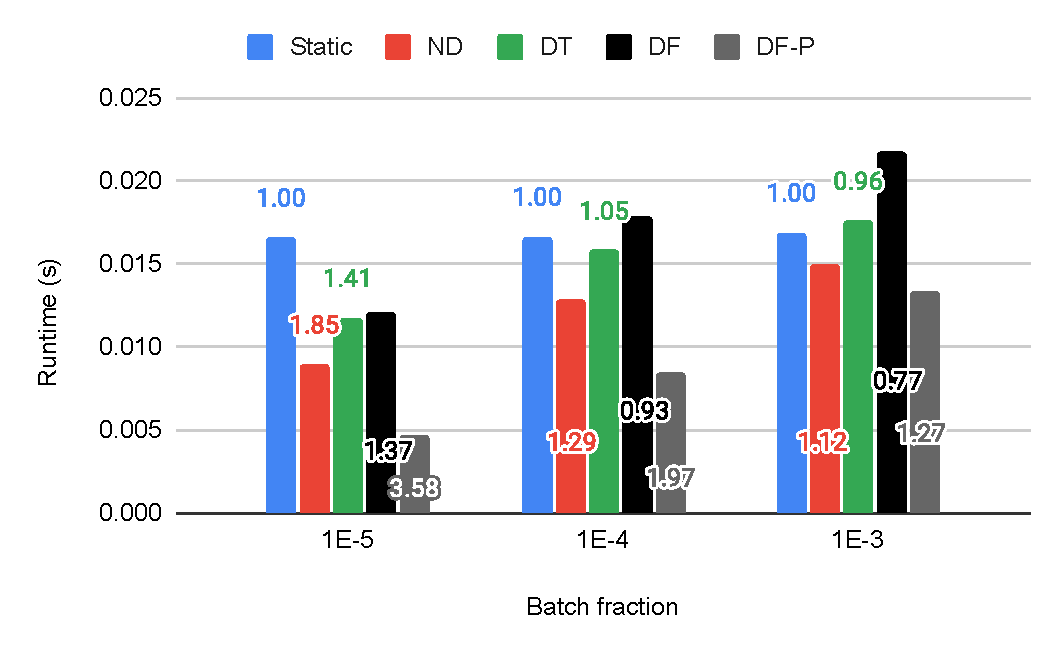
\includegraphics[width=0.48\linewidth]{out/temporal-summary-runtime-overall.pdf}
  }
  \subfigure[Overall Error in ranks obtained \textbf{(GPU)}]{
    \label{fig:temporal-compare--error-overall}
    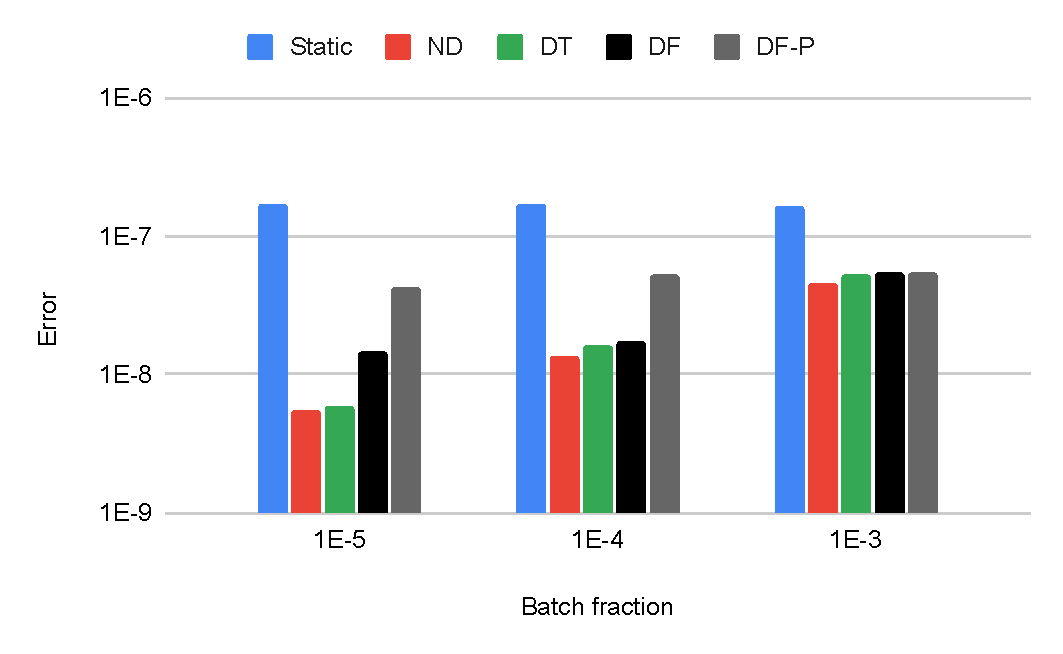
\includegraphics[width=0.48\linewidth]{out/temporal-summary-error-overall.pdf}
  }
  \subfigure[Overall Runtime \textbf{(CPU)}]{
    \label{fig:temporal-compare--runtime-overall-cpu}
    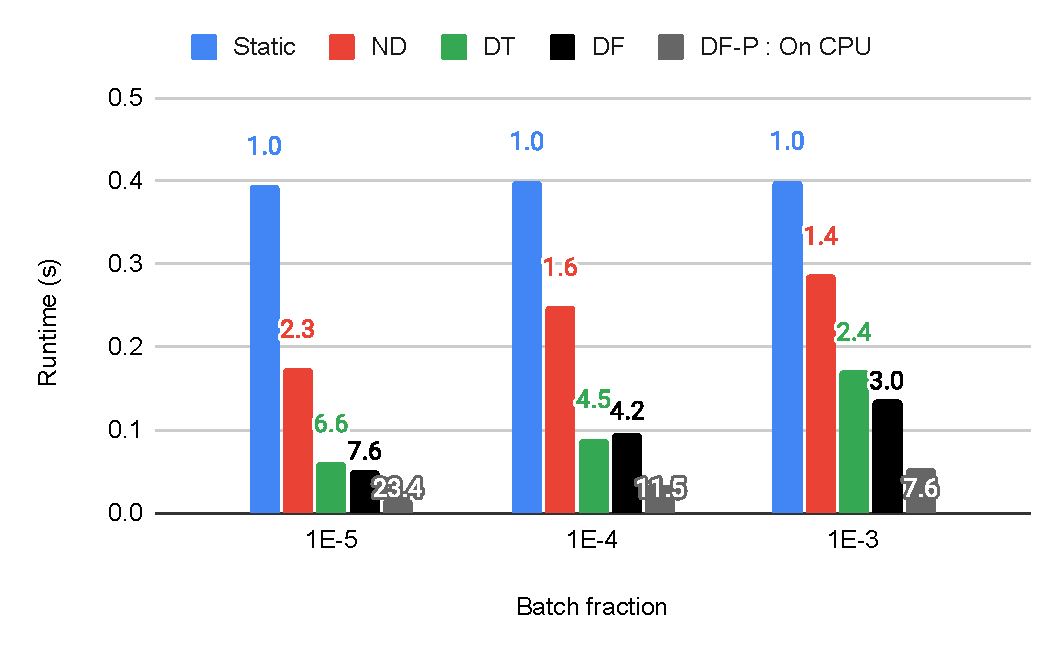
\includegraphics[width=0.48\linewidth]{out/temporal-summary-runtime-overall-cpu.pdf}
  }
  \subfigure[Overall Error in ranks obtained \textbf{(CPU)}]{
    \label{fig:temporal-compare--error-overall-cpu}
    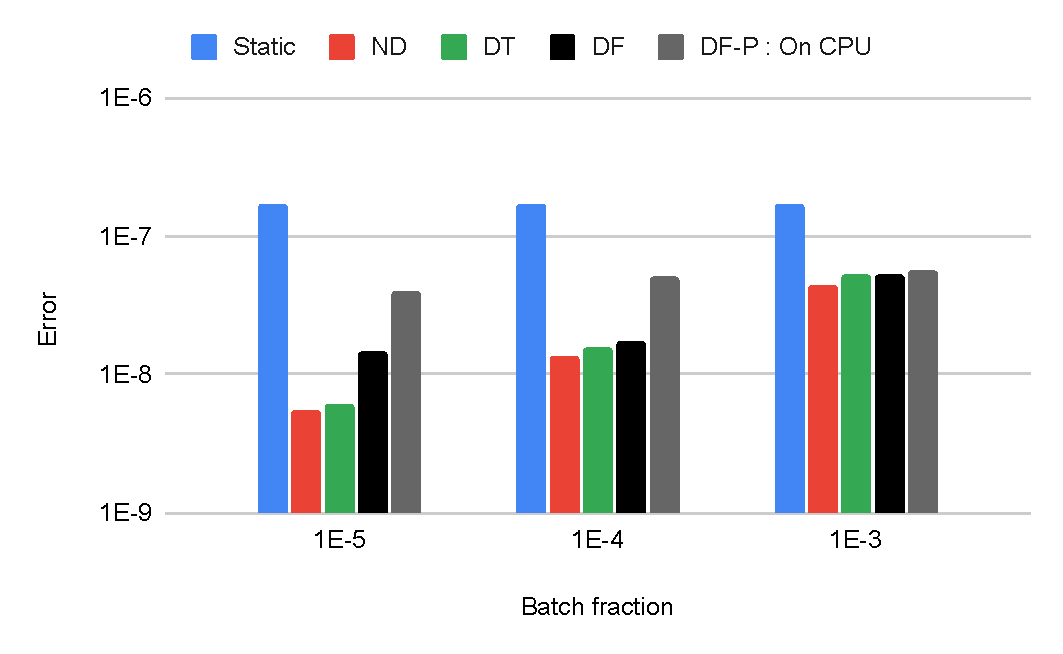
\includegraphics[width=0.48\linewidth]{out/temporal-summary-error-overall-cpu.pdf}
  } \\[-2ex]
  \caption{Mean Runtime and Error in ranks obtained with \textit{Static}, \textit{Naive-dynamic (ND)}, \textit{Dynamic Traversal (DT)}, our improved \textit{Dynamic Frontier (DF)}, and our improved \textit{Dynamic Frontier with Pruning (DF-P)} PageRank on real-world dynamic graphs, with batch updates of size $10^{-5}|E_T|$ to $10^{-3}|E_T|$. Here, (a) and (b) show the overall runtime and error across all temporal graphs, while (c) and (d) show the runtime and rank error for each approach (relative to reference Static PageRank, see Section \ref{sec:measurement}). In (a), the speedup of each approach with respect to Static PageRank is labeled. \su{TOWR}}
  \label{fig:temporal-compare}
\end{figure*}

\begin{figure*}[hbtp]
  \centering
  \subfigure[Overall result \textbf{(GPU)}]{
    \label{fig:8020-runtime-compare--mean}
    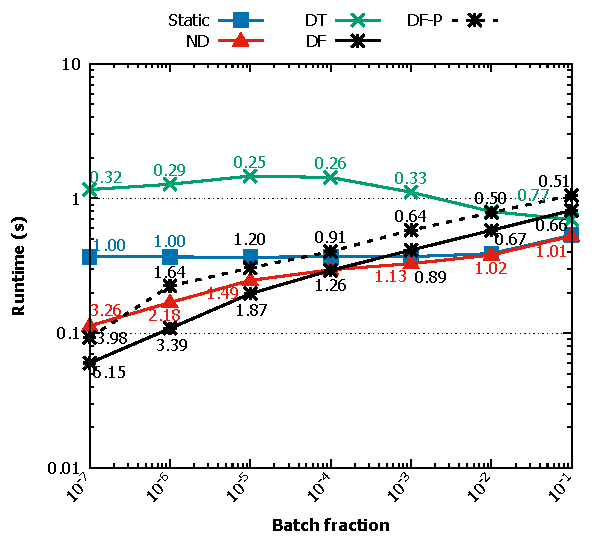
\includegraphics[width=0.38\linewidth]{out/8020-runtime-mean.pdf}
  }
  \subfigure[Results on each graph \textbf{(GPU)}]{
    \label{fig:8020-runtime-compare--all}
    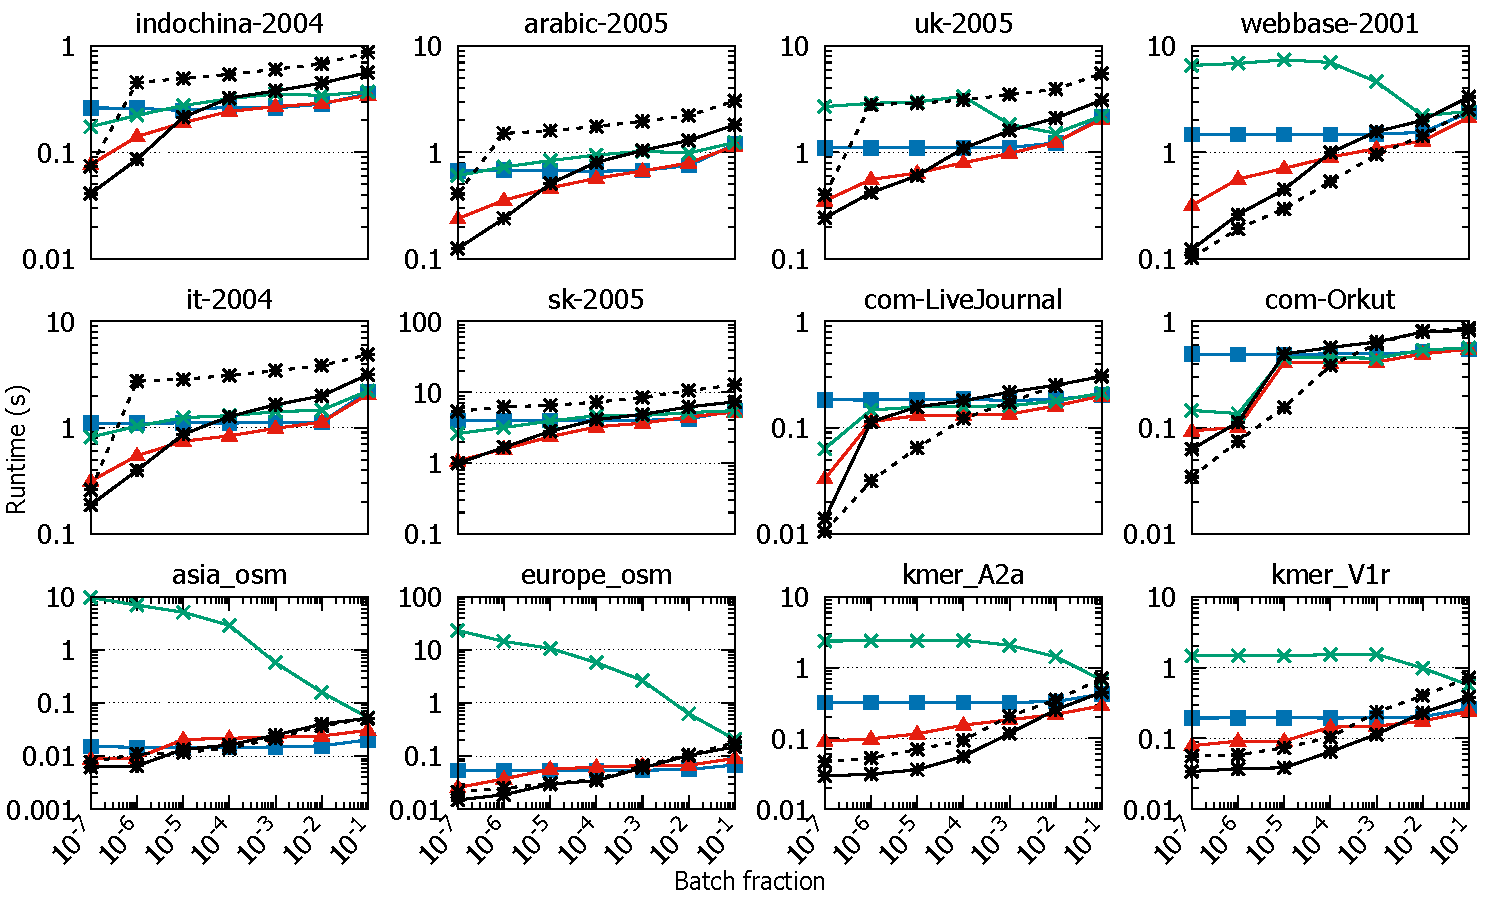
\includegraphics[width=0.58\linewidth]{out/8020-runtime-all.pdf}
  }
  \subfigure[Overall result \textbf{(CPU)}]{
    \label{fig:8020-runtime-compare--mean-cpu}
    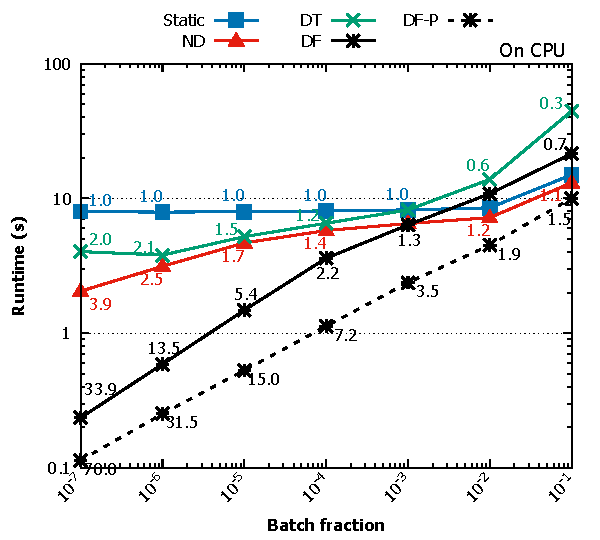
\includegraphics[width=0.38\linewidth]{out/8020-runtime-mean-cpu.pdf}
  }
  \subfigure[Results on each graph \textbf{(CPU)}]{
    \label{fig:8020-runtime-compare--all-cpu}
    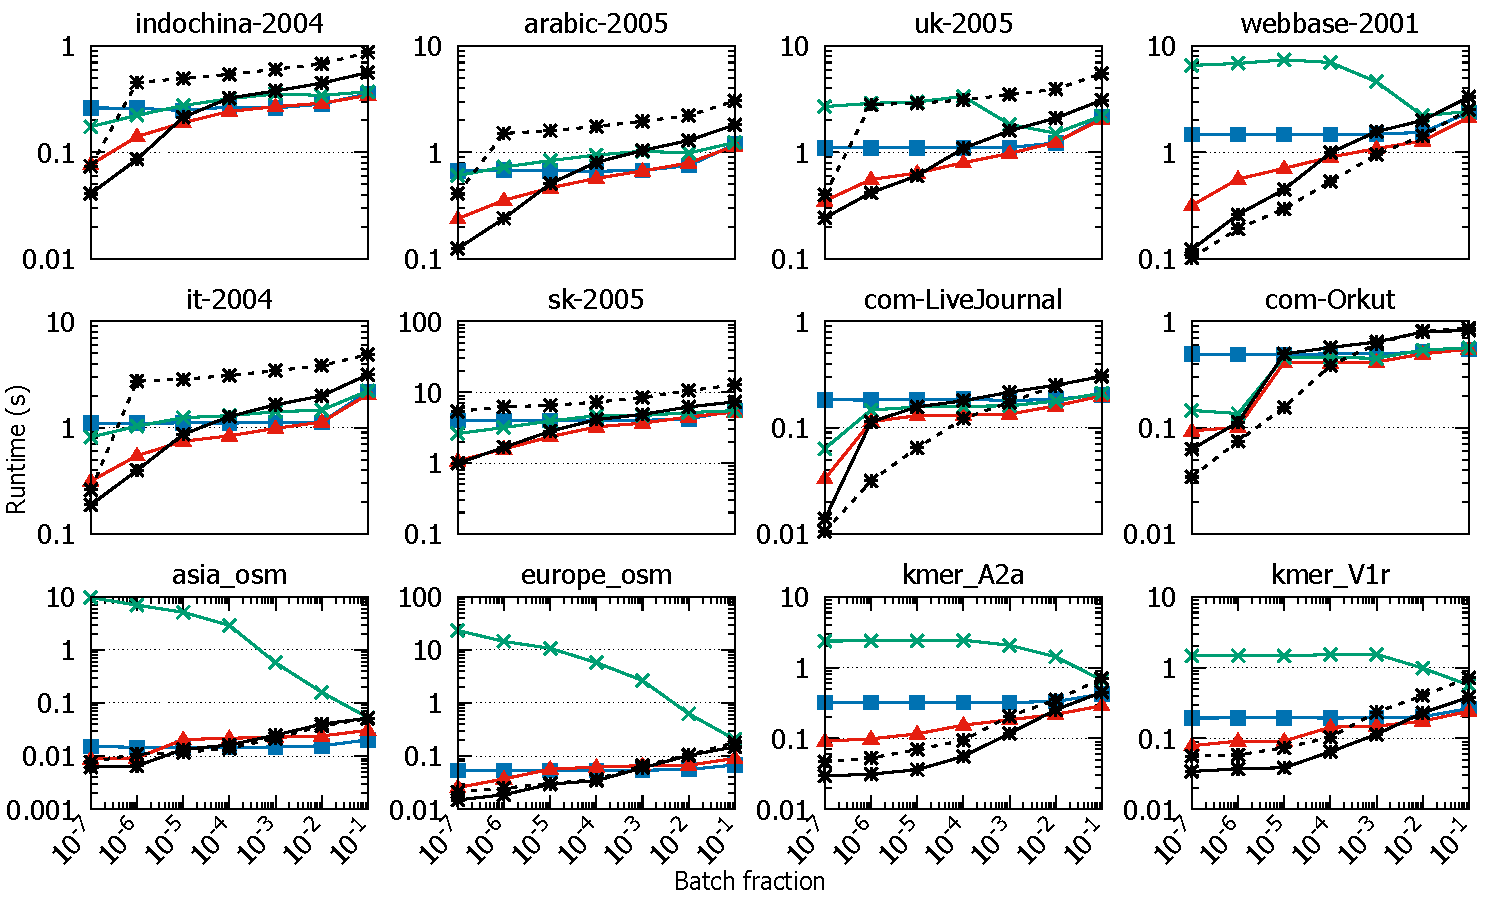
\includegraphics[width=0.58\linewidth]{out/8020-runtime-all.pdf}
  } \\[-1ex]
  \caption{Runtime (logarithmic scale) of our GPU implementation / multicore CPU implementation \cite{sahu2024df} of \textit{Static}, \textit{Naive-dynamic (ND)}, \textit{Dynamic Traversal (DT)}, \textit{Dynamic Frontier (DF)}, and \textit{Dynamic Frontier with Pruning (DF-P)} PageRank on large (static) graphs with generated random batch updates. Batch updates range in size from $10^{-7}|E|$ to $0.1|E|$ in multiples of $10$. These updates consist of $80\%$ edge insertions and $20\%$ edge deletions, mimicking realistic changes in a dynamic graph scenario. The right subfigures illustrate the runtime of each approach for individual graphs in the dataset, while the left subfigures present overall runtimes (using geometric mean for consistent scaling across graphs). Additionally, the speedup of each approach relative to Static PageRank is labeled on respective lines.}
  \label{fig:8020-runtime-compare}
\end{figure*}

\begin{figure*}[hbtp]
  \centering
  \subfigure[Overall result \textbf{(GPU)}]{
    \label{fig:8020-runtime-compare--mean}
    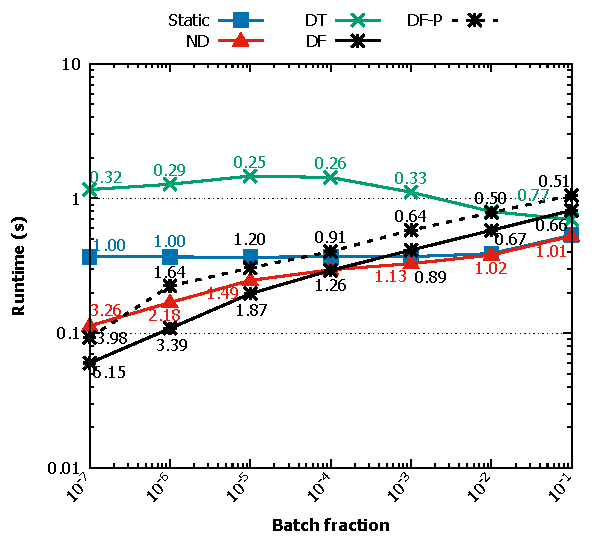
\includegraphics[width=0.38\linewidth]{out/8020-runtime-mean.pdf}
  }
  \subfigure[Results on each graph \textbf{(GPU)}]{
    \label{fig:8020-runtime-compare--all}
    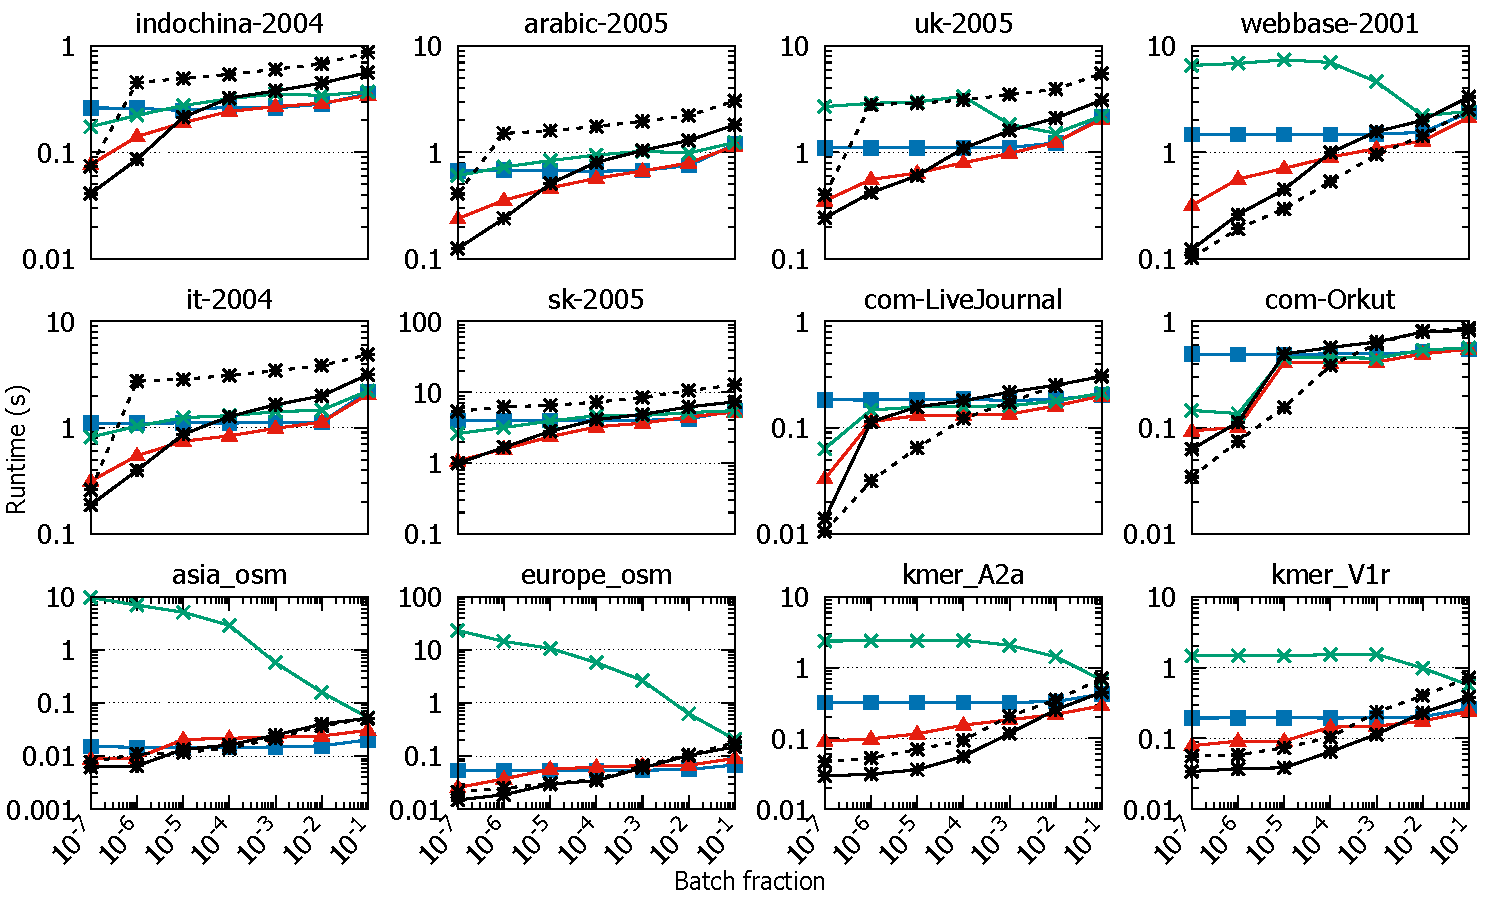
\includegraphics[width=0.58\linewidth]{out/8020-runtime-all.pdf}
  }
  \subfigure[Overall result \textbf{(CPU)}]{
    \label{fig:8020-runtime-compare--mean-cpu}
    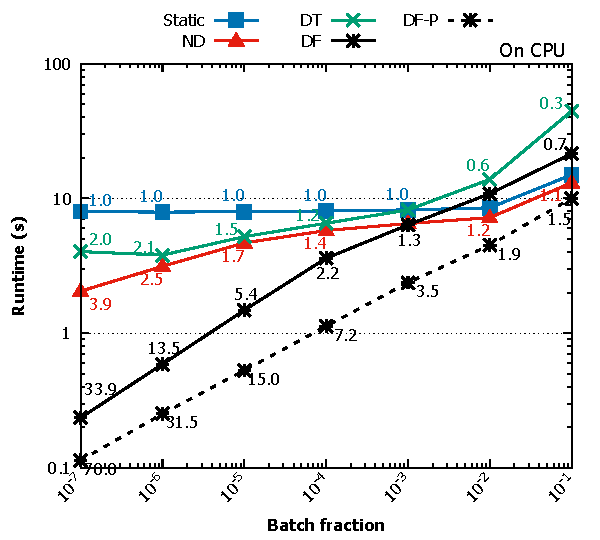
\includegraphics[width=0.38\linewidth]{out/8020-runtime-mean-cpu.pdf}
  }
  \subfigure[Results on each graph \textbf{(CPU)}]{
    \label{fig:8020-runtime-compare--all-cpu}
    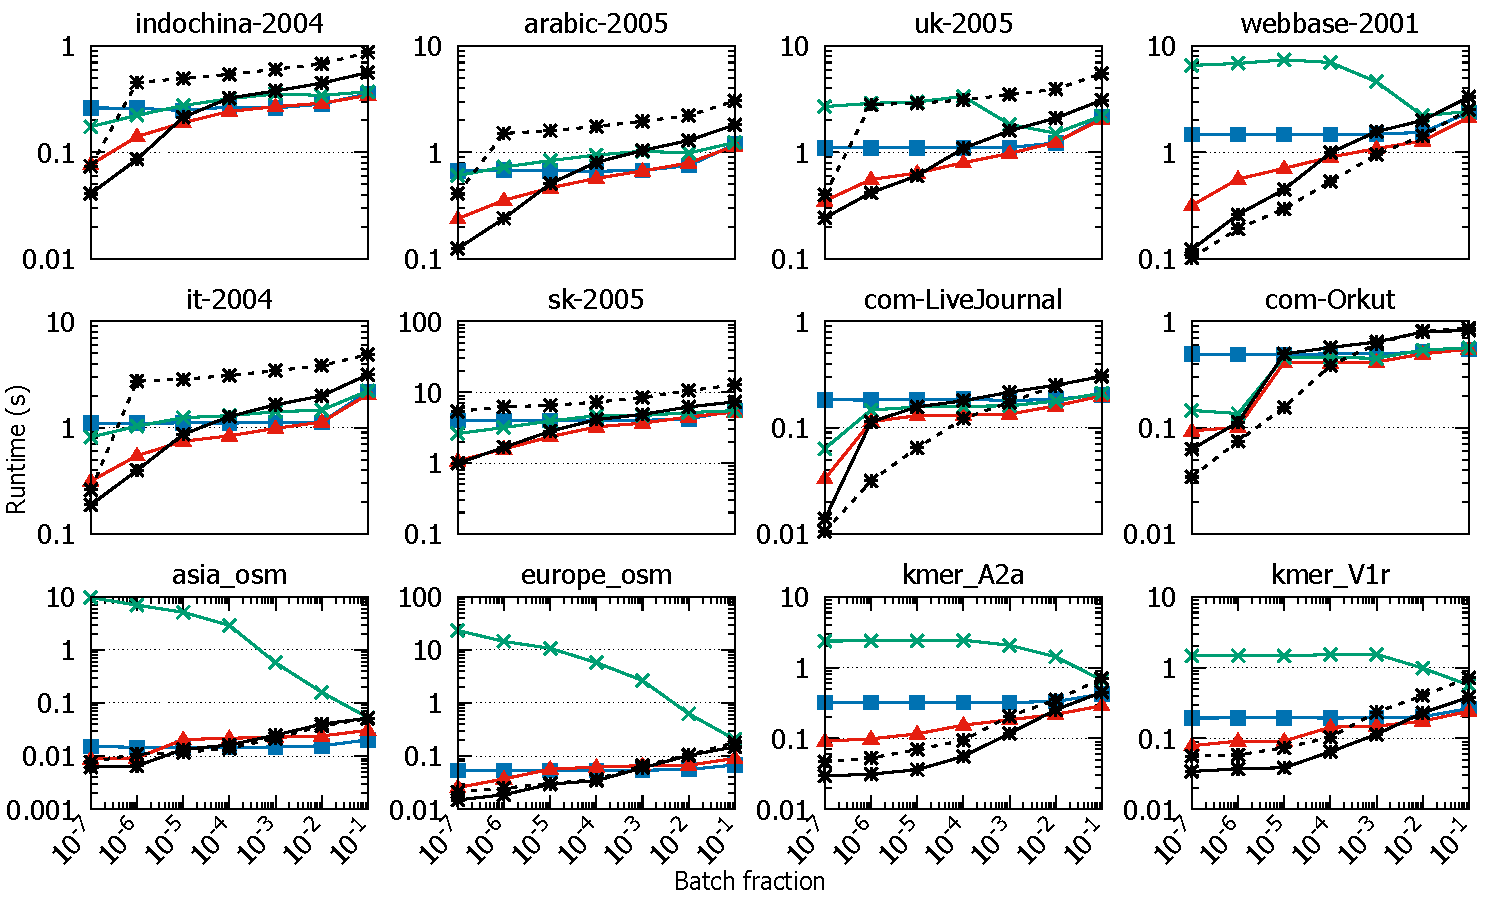
\includegraphics[width=0.58\linewidth]{out/8020-runtime-all.pdf}
  } \\[-1ex]
  \caption{Runtime (logarithmic scale) of our GPU implementation / multicore CPU implementation \cite{sahu2024df} of \textit{Static}, \textit{Naive-dynamic (ND)}, \textit{Dynamic Traversal (DT)}, \textit{Dynamic Frontier (DF)}, and \textit{Dynamic Frontier with Pruning (DF-P)} PageRank on large (static) graphs with generated random batch updates. Batch updates range in size from $10^{-7}|E|$ to $0.1|E|$ in multiples of $10$. These updates consist of $80\%$ edge insertions and $20\%$ edge deletions, mimicking realistic changes in a dynamic graph scenario. The right subfigures illustrate the runtime of each approach for individual graphs in the dataset, while the left subfigures present overall runtimes (using geometric mean for consistent scaling across graphs). Additionally, the speedup of each approach relative to Static PageRank is labeled on respective lines.}
  \label{fig:8020-runtime-compare}
\end{figure*}





\subsection{Indirect Comparison with State-of-the-art PageRank Implementations (Static)}

We now indirectly compare the performance of our GPU implementation of Static PageRank with other similar state-of-the-art implementations. Chen et al. \cite{chen2022atos} present Atos, a state-of-the-art task-parallel GPU scheduler for graph analytics. They say that in Gunrock and other frameworks, each frontier in a graph sweep is launched as a separate GPU kernel in the BSP model. This may result in insufficient parallelism, uneven finish times, and high kernel launch overhead for small frontiers. In contrast, Chen et al. present a persistent task scheduler which runs continuously to minimize kernel launch overhead, and also support asynchronous execution. For PageRank, they present a push-based asynchronous PageRank (requires many atomic ops) that uses a frontier to keep track of vertices that need to be processed in the next iteration. They use a queue to keep track fo the frontier (also requires atomic ops). Their CUDA kernel appears to be barrier-free. Their frontier concept is similar to ours \cite{sahu2024df}, but they do not use it for Dynamic PageRank. Chen et al. are able to achieve $3.2\times$ speedup over Gunrock on the \textit{indochina-2004} graph (see Table $1$ of their paper \cite{chen2022atos}). However, on the same graph, we achieve $24.4\times$ speedup over Gunrock (see Figure \ref{fig:compare--speedup} in this report).

In another work, Chen et al. \cite{chen2022scalable} extend their Atos dynamic scheduling framework to multi-node GPU systems that supports Partitioned Global Address Space (PGAS) style lightweight one-sided memory operations within and between nodes. However on the \textit{indochina-2004} graph, even with $4$ GPUs, they are unable to beat our speedup with respect to Gunrock (see Table $4$ of their paper \cite{chen2022scalable}, and Figure \ref{fig:compare--speedup} in this report).

Yang et al. \cite{yang2022graphblast} present GraphBLAST, A High-Performance Linear Algebra-based Graph Framework on the GPU. They discuss that GraphBLAS has lacked high-performance implementations for GPUs. Further, they say that GraphBLAS Template Library (GBTL), a GraphBLAS-inspired GPU graph framework, is an order of magnitude slower than state-of-the-art graph frameworks on the GPU in terms of performance. They say, the issue lies with the lack of generalizability of optimizations, irregular memory access patterns and load imbalance, and low compute-to-memory access ratio. Their new design principles include exploiting input sparsity, which allows users to write graph algorithms without specifying push and pull direction, exploiting output sparsity allows users to tell the backend which values of the output in a single vectorized computation they do not want computed, and load-balancing. For SpMV load balancing (like PageRank) they discuss two main approaches, row split, which seems like block-per-vertex; and merge-based, which seems like edge balanced between threads/blocks. For PageRank, they use merge-based load balancing with segmented scan. They also use a heuristic to switch between push- and pull-based approach. They say that the optimal time to switch from push to pull is very early on (as Ligra). On the \textit{indochina-2004} graph, they are able to achieve $2.2\times$/$1.2\times$ speedup over Gunrock (see Table $12$/$13$ in their paper \cite{yang2022graphblast}). However, on the same graph, we achieve $24.4\times$ speedup over Gunrock (see Figure \ref{fig:compare--speedup} in this report).

Wang et al. \cite{wang2021grus} present Grus, a Unified-memory-efficient High-performance Graph Processing on GPU. They focus on addressing the following, related to Unified Memory (UM): minimizing the amount of migrated data; reducing the number of page faults; and reducing page migration overhead. They achieve this with their framework with memory management and execution optimization. They use CSR as a space-efficient data structure for graph representation, and use $5|V|$ bytes for representing a frontier. They use an adaptive UM policy, where the frontier and ranks are assigned high priority, the CSR index array is assigned medium priority, and the CSR edges array is assigned low priority. They also use a Bitmap-directed frontier (8-bit integer array, similar to ours, plus a queue - no atomic ops needed), and use warp-centric load balancing (warp-per-vertex, similar to block-per-vertex, no partitioning) for PageRank computation. On the \textit{uk-2005} graph, they are able to achieve a $1.2\times$ speedup over Gunrock (see Table $4$ in their paper \cite{wang2021grus}). However, we get $8.6\times$ speedup over Gunrock on the same graph (see Figure \ref{fig:compare--speedup} in this report).

Concessao et al. \cite{concessao2023meerkat} propose a library-based framework for dynamic graph algorithms that utilizes a GPU-tailored graph representation and exploits the warp-cooperative execution model. The library, named Meerkat, builds upon a recently proposed dynamic graph representation on GPUs. This representation exploits a hashtable-based mechanism to store a vertex’s neighborhood. Meerkat also enables fast iteration through a group of vertices, such as the whole set of vertices or the neighbors of a vertex. They find that these two iteration patterns are common, and optimizing them is crucial for achieving performance. Meerkat supports dynamic edge additions and edge deletions, along with their batched versions. The PageRank implementation of Meerkat performs, on average, $1.7\times$ faster than Hornet. However, our Static PageRank is on average $31\times$ faster than Hornet (see Figure \ref{fig:compare--speedup} in our report).
